\documentclass{article}

\usepackage{amsfonts}
\usepackage{amsmath}
\usepackage{tikz}
\usetikzlibrary{calc, automata, chains, arrows.meta, math}
\usepackage{graphics}
\usepackage{float}
\usepackage{multicol}
\usepackage{mathtools}
\usepackage{xcolor}
\usepackage[toc, page]{appendix}
\usepackage{listings}

\usepackage{xcolor}

\definecolor{codegreen}{rgb}{0,0.6,0}
\definecolor{codegray}{rgb}{0.5,0.5,0.5}
\definecolor{codepurple}{rgb}{0.58,0,0.82}
\definecolor{backcolor}{rgb}{0.95,0.95,0.92}
\lstdefinestyle{pystyle}{
    backgroundcolor=\color{backcolor},
    commentstyle=\color{codegreen},
    keywordstyle=\color{magenta},
    numberstyle=\color{codegray},
    basicstyle=\ttfamily\footnotesize,
    breakatwhitespace=false,
    breaklines=true,
    captionpos=b,
    keepspaces=true,
    numbers=left,
    numbersep=5pt,
    showspaces=false,
    showstringspaces=false,
    showtabs=false,
    tabsize=2
}

\lstdefinestyle{terminalstyle}{
    basicstyle=\ttfamily\normalsize,
    captionpos=b,
    keepspaces=true,
}


\setcounter{MaxMatrixCols}{20}

\title{A game theoretic model of the behavioural gaming that takes place at the EMS - ED interface}
\author{Michalis Panayides}
\date{}

\begin{document}
    \maketitle
    \tableofcontents
    \newpage
    
    \section{Introduction}
    \section{Overview of game theoretic model}

The problem studied is a 3-player normal form game. The players are:
  
\begin{itemize}
    \item the decision makers of two queueing systems;
    \item a service that distributes individuals to these two queueing systems.
\end{itemize}

This is a standard Normal form game~\cite{Maschler2013},  
in that each player in this game has their own objectives which they aim to 
optimise.
More specifically, the queueing systems' objective is captured by an upper bound
of the time that a fixed proportion of individuals spend in the system, 
while the distributor aims to minimise the time that its individuals 
are blocked.
% TODO: Depending on how this is described earlier, we might need a little more 
% here (as to what we mean by "blocked")

The queueing systems are designed in such a way where they can accept two types
of individuals. 
These are the individuals that the distributor allocates to them and 
other individuals from other sources. 
Each queueing system may then choose to block the individuals that arrive from 
the distributor when the system reaches a certain capacity. 
The strategy sets for each queueing system is the set 
\( \{T \in \mathbb{N} \;|\; 1 \leq T \leq N\} \) where \(N \in\{N_A, N_B\}\) are 
the total capacities of the two queueing systems. We denote the chosen actions 
from the strategy set as \(T_A, T_B\) and call these \textit{threshold}s.

Both queueing systems follow a queueing model that has two waiting spaces for 
individuals. 
The first waiting zone is where the individuals queue right before receiving 
their service and has a capacity of \( N - C \), where \(N\) is the total 
capacity of the waiting space and \(C\) is the number of servers. 
The second waiting zone is where the individuals, that are sent from the 
distributor, remain until they are allowed to enter the first waiting zone.
The second waiting zone has a capacity of \(M\) and no servers.

This is shown diagrammatically in Figure ~\ref{fig:diagram_of_queueing_system}.

\begin{figure}[h]
    \centering
    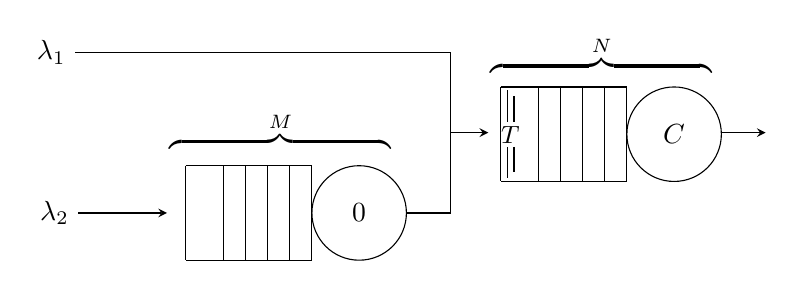
\begin{tikzpicture}[>=stealth, scale=0.8],
        % the rectangle of Queue 1
        \draw (0,0) -- ++(2cm,0) -- ++(0,-1.5cm) -- ++(-2cm,0);
        % The label above Queue 1 -> M
        \node[anchor=north] at (1.5cm, 1cm) {\( 
            \overbrace{\qquad \qquad \qquad \qquad}^{M} 
        \)};
        % the vertical lines in Queue 1
        \foreach \i in {1,...,4, 5.7}
        \draw (2cm-\i*10pt,0) -- +(0,-1.5cm);
        
        % the circle in Queue 1
        \draw (2.75,-0.75cm) circle [radius=0.75cm] node {\(0\)};

        % the rectangle in Queue 2
        \draw (5,1.25) -- ++(2cm,0) -- ++(0,-1.5cm) -- ++(-2cm,0);
        % the vertical lines in Queue 2
        \foreach \i in {1,...,4, 5.7}
        \draw (7cm-\i*10pt,1.25) -- +(0,-1.5cm);
        % The two vertical lines at the very start of Queue 2 
        \draw (7cm-54pt,1.2) -- +(0,-0.5cm);
        \draw (7cm-54pt,0.3) -- +(0,-0.5cm);        
        \draw (7cm-51pt,1.1) -- +(0,-0.4cm);
        \draw (7cm-51pt,0.3) -- +(0,-0.4cm);

        % The label between the lines for T
        \node[anchor=north] at (5.15, 0.77 cm) {\small{\( T \)}};

        % The label above Queue 2 -> N
        \node[anchor=north] at (6.6cm, 2.2cm) {\( 
            \overbrace{\qquad \qquad \qquad \qquad}^{N} 
        \)};

        % the circle in Queue 2
        \draw (7.75,0.5) circle [radius=0.75cm] node {\(C\)};

        % Arrow line from Queue 2 outside
        \draw[->] (8.5,0.525) -- +(20pt,0);
        
        % Line from lambda_2 to Queue 1
        \draw[<-] (-0.3,-0.75) -- +(-40pt,0) node[left] {\( \lambda_2 \)};
        % First line (horizontal) after Queue 1
        \draw[-] (3.5,-0.75) -- +(20pt,0);
        % Second line (vertical) after Queue 1
        \draw (4.2, 0.525) -- (4.2, -0.75);
        
        % First line (horizontal) from lambda_1
        \draw (4.2, 1.8) -- +(-169.5pt,0) node[left] {\( \lambda_1 \)};
        % Second line (vertical) from lambda_1
        \draw (4.2, 1.8) -- (4.2, 0.525);
        % Arrow line to Queue 2
        \draw[->] (4.2, 0.525) -- (4.8, 0.525);  
    \end{tikzpicture}
    \caption{A diagrammatic representation of the queueing model. 
    The threshold \(T\) only applies to arrivals from the first buffer. 
    If the second buffer is at that threshold only individuals of the first type 
    are accepted (at a rate \(\lambda_1\)) and individuals of the second type 
    (arriving at a rate \(\lambda_2\)) are held blocked in the first buffer.}
    \label{fig:diagram_of_queueing_system}
\end{figure}

Note here that both types of individuals can become lost to the system. 
Individual allocated from the distributor become lost to the system whenever 
an arrival occurs and the second waiting zone is at full capacity (\(M\) 
individuals already waiting).
Similarly, other individuals get lost whenever they arrive at the first waiting 
zone and it is at full capacity (\(N - C\) individuals already waiting).

Following this queuing model, the two queueing systems' choice of strategy will 
then rely solely on satisfying their own 
objective, which is to make sure that the waiting time in the first waiting zone 
of a proportion of individuals will be below the predefined target time.

\begin{equation}
    P(W < R) \geq \hat{P}
\end{equation}

where \(W\) is the mean waiting time of all individuals, \(R\) is the time 
target and \(\hat{P}\) is the percentage of individuals need to be within that 
target. 
There are numerous objective functions that can be used to capture this 
behaviour. 
For example one approach is to use the threshold that maximises the probability 
that 
the mean waiting is more than the target time, and completely ignore the 
percentage goal.

\begin{equation}
    \arg \max_{T_i} \quad P(W_i < R)
\end{equation}

A more sophisticated objective function would be to get the proportion 
of individuals as close to the percentage aim. 
In other words, to find the threshold that minimises the difference between the 
probability and the percentage goal (or maximise its negation).

\begin{equation}\label{eq:obj-queueing-systems}
    \arg \max_{T_i} \quad -\left( \hat{P} - P(W_i < R) \right)^2
\end{equation}


The third player, the distributor has their own choices to make and their own 
goals to satisfy.
The strategy set of the third player is the proportion \(0 \leq p \leq 1\) of 
individuals it sends to the first queueing system (the proportion \(1 - q\) is 
sent to the second queueing system).
In addition, the distributor aims to minimise any potential blockages
that may occur, given the pair of thresholds chosen by the two queueing systems.
Thus, its objective is to minimise the blocked time of the individuals 
that they send to the two queueing systems.
Apart from the time being blocked, an additional aspect that may affect the 
decision of the distributor is the proportion of lost individuals.
Equation \ref{eq:obj-distributor} can be used to capture a mixture 
between the two objectives.

\begin{equation}\label{eq:obj-distributor}
    \alpha P(L_A) + (1 - \alpha) B_A = 
    \alpha P(L_B) + (1 - \alpha) B_B
\end{equation}

Here, \(\alpha\) represents the ``importance'' of each objective,
where high \(\alpha\) indicates a higher weight on the proportion of lost 
individuals and smaller \(\alpha\) a higher weight on the time blocked. 


Using equations \ref{eq:obj-queueing-systems} and \ref{eq:obj-distributor} gives
an imperfect information extensive form game. 
An imperfect information game is defined as an extensive form game where some 
of the information about the game state is hidden for at least one of the 
players~\cite{Berwanger2008}. In this study the state of the problem that is
hidden is the threshold that each of the first two players chooses to play.
In other words, each queueing system chooses to play a strategy without the 
knowing the other system's strategy.
The distributor then, fully aware of the chosen threshold strategies, distributes 
individuals among the two systems in order to minimise the time that its 
individuals will be blocked. Figure \ref{fig:imperfect-info-game} illustrates this. 

\begin{figure}[ht]
    \centering
    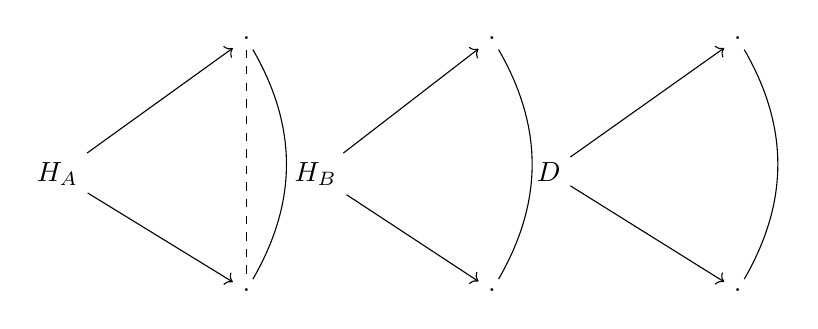
\begin{tikzpicture}[-, node distance = 3cm, scale=0.8]
        \node[anchor=north](HA){\(H_A\)};
        \node[anchor=north](HA_d1) at (3, 2){.};
        \node[anchor=north](HA_d2) at (3, -2){.};
    
        \path[->] (HA) edge node {}(HA_d1);
        \path[->] (HA) edge node {}(HA_d2);
        \path (HA_d1) edge [bend left] node {}(HA_d2);
        \path (HA_d1) [dashed] edge node {}(HA_d2);
    
        \node[anchor=north](HB) at (4.1, 0){\(H_B\)};
        \node[anchor=north](HB_d1) at (6.9, 2){.};
        \node[anchor=north](HB_d2) at (6.9, -2){.};
    
        \path[->] (HB) edge node {}(HB_d1);
        \path[->] (HB) edge node {}(HB_d2);
        \path(HB_d1) edge [bend left] node {}(HB_d2);
    
        \node[anchor=north](D) at (7.8, 0){\(D\)};
        \node[anchor=north](D_d1) at (10.8, 2){.};
        \node[anchor=north](D_d2) at (10.8, -2){.};
        
        \path[->] (D) edge node {}(D_d1);
        \path[->] (D) edge node {}(D_d2);
        \path(D_d1) edge [bend left] node {}(D_d2);
    \end{tikzpicture}
    \caption{Imperfect information Extensive Form Game between the distributor 
    and the 2 queueing systems}
    \label{fig:imperfect-info-game}
\end{figure}

The first 
queueing system \(H_A\) decides on a threshold, then the second system \(H_B\)
chooses its own threshold, without knowing the strategy of \(H_A\), and finally
the distributor makes its choice. Note here that the dotted line represents the
fact that \(H_B\) is unaware of the state of the game when making its own 
decisions. The game can thus be partitioned into a normal form game between the
two queueing systems and finding the distributor's best choice. 

In order to define the normal form game the two payoff matrices of the players 
are required. From equation \ref{eq:obj-queueing-systems} the utilities of the
players can be formulated as:

\begin{equation}
    U_{T_1, T_2}^i = \quad -\left( 
        \hat{P} - P(W_i < R) 
    \right)^2
\end{equation}

Consequently, the payoff matrices of the game can be populated by these 
utilities:

\begin{equation} \label{eq:payoff-matrices}
    A = 
    \begin{pmatrix}
        U_{1,1}^A & U_{1,2}^A & \dots & U_{1,N_B}^A \\
        U_{2,1}^A & U_{2,2}^A & \dots & U_{2,N_B}^A \\
        \vdots & \vdots & \ddots & \vdots \\
        U_{N_A,1}^A & U_{N_A,2}^A & \dots & U_{N_A,N_B}^A \\
    \end{pmatrix},
    B = 
    \begin{pmatrix}
        U_{1,1}^B & U_{1,2}^B & \dots & U_{1,N_B}^B \\
        U_{2,1}^B & U_{2,2}^B & \dots & U_{2,N_B}^B \\
        \vdots & \vdots & \ddots & \vdots \\
        U_{N_A,1}^B & U_{N_A,2}^B & \dots & U_{N_A,N_B}^B \\
    \end{pmatrix}
\end{equation}

Based on the choice of strategy of these two players the distributor will then 
make their own choice of the proportion of individuals to send to each system.

    \section{A queueing model with 2 consecutive buffer centres}

% TODO: If this is to be one paper maybe the first two paragraphs do not need to
% include so much details or even better omit some of the details in the game
% overview section.
In this section, a more in-depth explanation of the queueing model shown in 
figure \ref{fig:diagram_of_queueing_system} will be given.
This is a queuing model that consists of two waiting spaces, one for each type
of individual.

The model consists of two types of individuals; class 1 and class 2.
Class 1 individuals arrive instantly at waiting zone 1 and proceed to wait to
receive their service. 
Class 2 individuals arrive at waiting zone 2 and wait there until they are 
allowed to move to waiting zone 1. 
They are allowed to proceed only when the number of 
individuals in waiting zone 1 \textbf{and} in service is less than a 
pre-determined threshold \(T\).
When the number of individuals is equal to or exceeds this threshold, all second type individuals that arrive will remain 
\textit{``blocked''} in waiting zone 1 until the number of people in the 
system is reduced below \(T\). 
This is shown diagrammatically in figure \ref{fig:diagram_of_queueing_system}.
The parameters of the described queueing model are:

\begin{itemize}
    \item \(\lambda_i\): The arrival rate of individuals of type \(i\in\{1, 2\}\)
    \item \(\mu\): The service rate for individuals receiving service
    \item \(C\): The number of servers
    \item \(T\): The threshold at which individuals of the second type are blocked
\end{itemize}

Under the assumption that all rates (arrival and service) are Markovian the
queuing system corresponds to a Markov chain~\cite{kemeny1976markov}.
The states of the Markov chain are denoted by \((u,v)\) where:

\begin{itemize}
    \item \(u\) is the number of individuals blocked
    \item \(v\) is the number of individuals either in waiting zone 1 or in the
    service centre
\end{itemize}

We denote the state space of the Markov chain as  \(S=S(T)\) which can be 
written as the disjoint union (\ref{eq:definition_of_S_as_disjoint_union}).

\begin{align}
    S(T) =& S_1(T) \cup S_2(T) \text{ where:} \nonumber \\
    S_1(T) =& \left\{(0, v)\in\mathbb{N}_0^2 \; | \; v < T \right\} 
    \label{eq:definition_of_S_as_disjoint_union} \\
    S_2(T) =& \{(u, v)\in\mathbb{N}_0^2 \; | \; v \geq T \} \nonumber
\end{align}

The transition matrix \(Q\) of the Markov chain consists of the transition rates
between the numerous states of the model. Every entry \( Q_{ij} = 
Q_{(u_i, v_i),(u_j, v_j)} \) represents the transition rate from state 
\( i = (u_i, v_i) \) to state \( j = (u_j , v_j) \) for all 
\( (u_i, v_i), (u_j, v_j) \in S \).
The entries of \(Q\) can be calculated using the state-mapping function 
described in (\ref{eq:markov_transition_rate}): 

\begin{equation} \label{eq:markov_transition_rate}
    Q_{ij} = 
    \begin{cases}
        \Lambda, & \textbf{if } (u_i, v_i) - (u_j, v_j) = (0,-1) \textbf{ and } 
        v_i < \text{t} \\
        \lambda_1, & \textbf{if } (u_i, v_i) - (u_j, v_j) = (0,-1) 
        \textbf{ and } v_i \geq \text{t} \\
        \lambda_2, & \textbf{if } (u_i, v_i) - (u_j, v_j) = (-1,0) \\
        v_i \mu, & \textbf{if } (u_i, v_i) - (u_j, v_j) = (0,1) \textbf{ and } 
        v_i \leq C \textbf{ or} \\ & \hspace{0.37cm}(u_i, v_i) - (u_j, v_j) = 
        (1,0) \textbf{ and } v_i = T \leq C \\
        C \mu, & \textbf{if } (u_i, v_i) - (u_j, v_j) = (0,1) \textbf{ and } 
        v_i > C 
        \textbf{ or} \\ & \hspace{0.37cm}(u_i, v_i) - (u_j, v_j) = (1,0) 
        \textbf{ and } v_i = T > C\\
        -\sum_{j=1}^{|Q|}{Q_{ij}} & \textbf{if } i = j \\
        0, & \textbf{otherwise}
    \end{cases}
\end{equation}

Note that \(\Lambda\) here denotes the overall arrival rate in the model by both 
classes of individuals (i.e. \(\Lambda = \lambda_1 + \lambda_2\)). 
A visualisation of how the transition rates relate to the states of the model 
can be seen in the general Markov chain model shown in figure 
\ref{fig:general-markov-model}.

\begin{figure}[H]
    \centering
    \scalebox{.8}
    {
        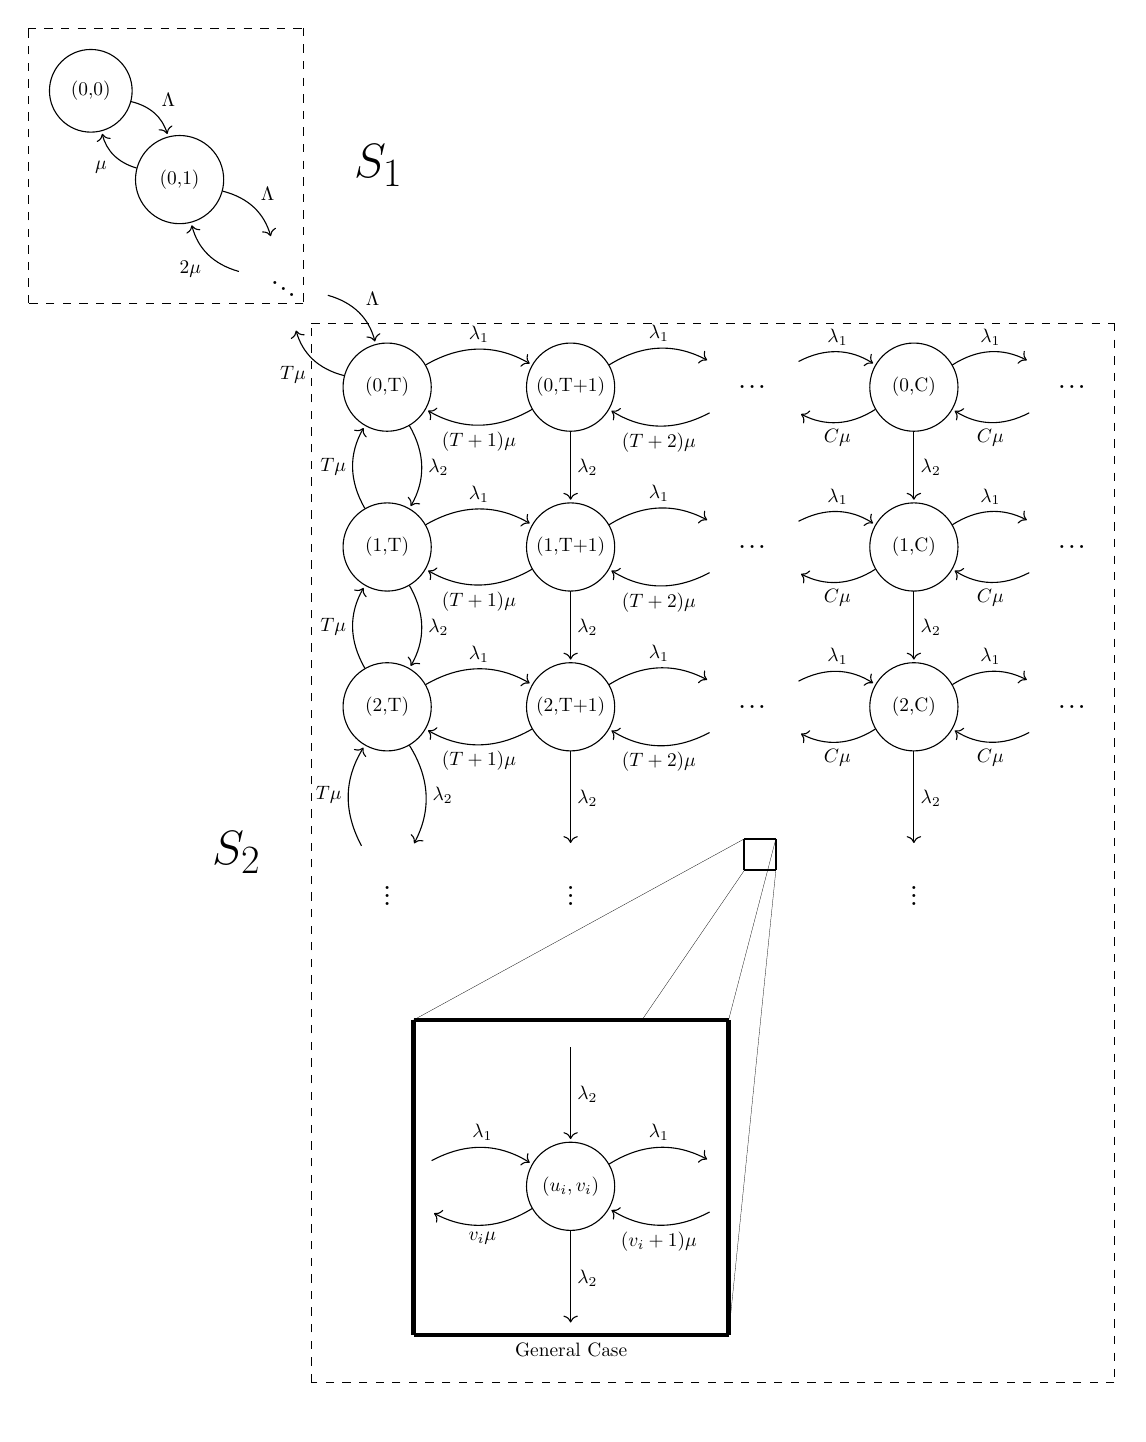
\begin{tikzpicture}[-, node distance = 0.9cm, auto, every node/.style={scale=0.7}]

            % Markov chain variables
            \tikzmath{
                let \initdist = 0.5cm;
                let \altdist = 1.2cm;
                let \minsz = 1.6cm;
            }

            % S_1 and S_2 rectangles
            \tikzmath{
                let \leftOne = -0.8;
                let \rightOne = 2.7;
                let \upOne = 0.8;
                let \downOne = -2.7;
                let \leftTwo = 2.8;
                let \rightTwo = 13;
                let \upTwo = -2.95;
                let \downTwo = -16.4;
            }

            % General case variables
            \tikzmath{
                let \GCsmallx = 8.3;
                let \GCsmally = -9.5;
                let \GCbigx = 4.1;
                let \GCbigy = -11.8;
            }

            % Rectangle for S1
            \draw[ultra thin, dashed] (\leftOne, \downOne) -- (\leftOne, \upOne);
            \draw[ultra thin, dashed] (\leftOne, \upOne) -- (\rightOne, \upOne);
            \draw[ultra thin, dashed] (\rightOne, \upOne) -- node 
            {\Huge{\( \quad S_1 \)}}(\rightOne, \downOne);
            \draw[ultra thin, dashed] (\rightOne, \downOne) -- (\leftOne, \downOne);

            % Rectangle for S2
            \draw[ultra thin, dashed] (\leftTwo, \downTwo) -- node 
            {\Huge{\( S_2 \quad \)}}(\leftTwo, \upTwo);
            \draw[ultra thin, dashed] (\leftTwo, \upTwo) -- (\rightTwo, \upTwo);
            \draw[ultra thin, dashed] (\rightTwo, \upTwo) -- (\rightTwo, \downTwo);
            \draw[ultra thin, dashed] (\rightTwo, \downTwo) -- (\leftTwo, \downTwo);

            % Small square of general case
            \draw [thick] (\GCsmallx, \GCsmally) -- node {} 
            (\GCsmallx + 0.4, \GCsmally);
            \draw [thick] (\GCsmallx + 0.4, \GCsmally) -- node {} 
            (\GCsmallx + 0.4, \GCsmally - 0.4);
            \draw [thick] (\GCsmallx + 0.4, \GCsmally - 0.4) -- node {} 
            (\GCsmallx, \GCsmally - 0.4);
            \draw [thick] (\GCsmallx, \GCsmally - 0.4) -- node {} 
            (\GCsmallx, \GCsmally);


            % Dashed lines to from small square to big one 
            \draw [ultra thin] (\GCsmallx, \GCsmally) -- node {} 
            (\GCbigx, \GCbigy);
            \draw [ultra thin] (\GCsmallx + 0.4, \GCsmally) -- node {} 
            (\GCbigx + 4, \GCbigy);
            \draw [ultra thin] (\GCsmallx, \GCsmally - 0.4) -- node {} (7, \GCbigy);
            \draw [ultra thin] (\GCsmallx + 0.4, \GCsmally - 0.4) -- node {} 
            (\GCbigx + 4, \GCbigy - 4);
            
            % Big Square of general case
            \draw [ultra thick] (\GCbigx, \GCbigy) -- node {} (\GCbigx + 4, \GCbigy);
            \draw [ultra thick] (\GCbigx + 4, \GCbigy) -- node {} 
            (\GCbigx + 4, \GCbigy - 4);
            \draw [ultra thick] (\GCbigx + 4, \GCbigy - 4) -- node {General Case} 
            (\GCbigx, \GCbigy - 4);
            \draw [ultra thick] (\GCbigx, \GCbigy - 4) -- node {} (\GCbigx, \GCbigy);

            % First Line
            \node[state, minimum size=1.5cm] (zero) {(0,0)};
            \node[state, node distance = \initdist, minimum size=\minsz, below right=of zero] 
            (one) {(0,1)};
            \node[draw=none, node distance = \initdist, minimum size=\minsz, below right=of one] 
            (two) {\textbf{\( \ddots \)}};
            \node[state, node distance = \initdist, minimum size=\minsz, below right=of two] 
            (three) {(0,T)};
            \node[state, node distance = \altdist, minimum size=\minsz, right=of three] 
            (four) {(0,T+1)};
            \node[draw=none, node distance = \altdist, minimum size=\minsz, right=of four] 
            (five) {\textbf{\dots}};
            \node[state, minimum size=\minsz, right=of five] (six) {(0,C)};
            \node[draw=none, minimum size=\minsz, right=of six] (seven) {\textbf{\dots}};

            % Second Line
            \node[state, minimum size=\minsz, below=of three] (three_one) {(1,T)};
            \node[state, minimum size=\minsz, below=of four] (four_one) {(1,T+1)};
            \node[draw=none, minimum size=\minsz, below=of five] (five_one) {\textbf{\dots}};
            \node[state, minimum size=\minsz, right=of five_one] (six_one) {(1,C)};
            \node[draw=none, minimum size=\minsz, right=of six_one] (seven_one) {\textbf{\dots}};
            
            % Third Line
            \node[state, minimum size=\minsz, below=of three_one] (three_two) {(2,T)};
            \node[state, minimum size=\minsz, below=of four_one] (four_two) {(2,T+1)};
            \node[draw=none, minimum size=\minsz, below=of five_one] (five_two) 
            {\textbf{\dots}};
            \node[state, minimum size=\minsz, right=of five_two] (six_two) {(2,C)};
            \node[draw=none, minimum size=\minsz, right=of six_two] (seven_two) 
            {\textbf{\dots}};

            % Fourth line
            \node[draw=none, node distance = \altdist, minimum size=\minsz, below=of three_two] 
            (three_three) {\textbf{\vdots}};
            \node[draw=none, node distance = \altdist, minimum size=\minsz, below=of four_two] 
            (four_three) {\textbf{\vdots}};
            \node[draw=none, node distance = 2cm, minimum size=\minsz, below=of five_two] 
            (five_three) {};
            \node[draw=none, node distance = \altdist, minimum size=\minsz, below=of six_two] 
            (six_three) {\textbf{\vdots}};

            % Fifth line
            \node[draw=none, node distance = 0.3cm, minimum size=\minsz, below=of four_three] 
            (general_case_up) {};
            \node[state, node distance = \altdist, minimum size=\minsz, below=of general_case_up] 
            (general_case_mid) {\( (u_i, v_i) \)};

            \node[draw=none, node distance = \altdist, minimum size=\minsz, below=of general_case_mid] 
            (general_case_down) {};
            \node[draw=none, node distance = \altdist, minimum size=\minsz, left=of general_case_mid] 
            (general_case_left) {};
            \node[draw=none, node distance = \altdist, minimum size=\minsz, right=of general_case_mid] 
            (general_case_right) {};

            \draw[every loop]
                % First Horizontal Edges
                (zero) edge[bend left] node {\( \Lambda \)} (one)
                (one) edge[bend left] node {\( \mu \)} (zero)
                (one) edge[bend left] node {\( \Lambda \)} (two)
                (two) edge[bend left] node {\( 2 \mu \)} (one)
                (two) edge[bend left] node {\( \Lambda \)} (three)
                (three) edge[bend left] node {\( T \mu \)} (two)
                (three) edge[bend left] node {\( \lambda_1 \)} (four)
                (four) edge[bend left] node {\( (T+1) \mu \)} (three)
                (four) edge[bend left] node {\( \lambda_1 \)} (five)
                (five) edge[bend left] node {\( (T+2) \mu \)} (four)
                (five) edge[bend left] node {\( \lambda_1 \)} (six)
                (six) edge[bend left] node {\( C\mu \)} (five)
                (six) edge[bend left] node {\( \lambda_1 \)} (seven)
                (seven) edge[bend left] node {\( C\mu \)} (six)

                % Second Horizontal Edges
                (three_one) edge[bend left] node {\( \lambda_1 \)} (four_one)
                (four_one) edge[bend left] node {\( (T+1) \mu \)} (three_one)
                (four_one) edge[bend left] node {\( \lambda_1 \)} (five_one)
                (five_one) edge[bend left] node {\( (T+2) \mu \)} (four_one)
                (five_one) edge[bend left] node {\( \lambda_1 \)} (six_one)
                (six_one) edge[bend left] node {\( C\mu \)} (five_one)
                (six_one) edge[bend left] node {\( \lambda_1 \)} (seven_one)
                (seven_one) edge[bend left] node {\( C\mu \)} (six_one)

                % Third Horizontal Edges
                (three_two) edge[bend left] node {\( \lambda_1 \)} (four_two)
                (four_two) edge[bend left] node [below] {\( (T+1) \mu \)} (three_two)
                (four_two) edge[bend left] node {\( \lambda_1 \)} (five_two)
                (five_two) edge[bend left] node {\( (T+2) \mu \)} (four_two)
                (five_two) edge[bend left] node {\( \lambda_1 \)} (six_two)
                (six_two) edge[bend left] node {\( C\mu \)} (five_two)
                (six_two) edge[bend left] node {\( \lambda_1 \)} (seven_two)
                (seven_two) edge[bend left] node {\( C\mu \)} (six_two)

                % First Vertical Edges
                (three) edge[bend left] node {\( \lambda_2 \)} (three_one)
                (three_one) edge[bend left] node {\( T \mu \)} (three)
                (three_one) edge[bend left] node {\( \lambda_2 \)} (three_two)
                (three_two) edge[bend left] node {\( T\mu \)} (three_one)
                (three_two) edge[bend left] node {\( \lambda_2 \)} (three_three)
                (three_three) edge[bend left] node {\( T\mu \)} (three_two)

                % Second Vertical Edges
                (four) edge node {\( \lambda_2 \)} (four_one)
                (four_one) edge node {\( \lambda_2 \)} (four_two)
                (four_two) edge node {\( \lambda_2 \)} (four_three)

                % Fourth Vertical Edges
                (six) edge node {\( \lambda_2 \)} (six_one)
                (six_one) edge node {\( \lambda_2 \)} (six_two)
                (six_two) edge node {\( \lambda_2 \)} (six_three)

                % General Case
                (general_case_left) edge[bend left] node {\( \lambda_1 \)} (general_case_mid)
                (general_case_mid) edge[bend left] node {\( v_i \mu \)} (general_case_left)
                (general_case_right) edge[bend left] node {\( (v_i +1) \mu \)} (general_case_mid)
                (general_case_mid) edge[bend left] node {\( \lambda_1 \)} (general_case_right)
                % (five_three) edge node {\( \lambda_2 \)} (general_case_mid)
                (general_case_up) edge node {\( \lambda_2 \)} (general_case_mid)
                (general_case_mid) edge node {\( \lambda_2 \)} (general_case_down)
                ;
        \end{tikzpicture}
    }
    \caption{General case of the Markov chain model} 
    \label{fig:general-markov-model}
\end{figure}



In order to consider this model numerically an adjustment needs to be made. 
The problem defined above assumes no upper boundary to the number of individuals 
that can wait for service or for the ones that are blocked in the buffer centre. 
Therefore, a different state space \( \tilde S \) is constructed where 
\( \tilde S \subseteq S \) and there is a maximum allowed number of individuals 
\(N\) that can be in the system and a maximum allowed number of individuals 
\(M\) that can be blocked in the buffer centre:

\begin{equation}
    \tilde S = \left\{ (u, v) \in S\;| u \leq M, v\leq N \right\}
\end{equation}


\subsection{Performance Measures}


The transition matrix \( Q \) defined in \ref{eq:markov_transition_rate} can be 
used to get the probability vector \( \pi \).
The vector \( \pi \) is commonly used to study stochastic systems and it's main
purpose is to keep track of the probability of being at any given state of 
the system.
The term \textit{steady state} refers to the instance of the vector \( \pi \) 
where the probabilities of being at any state become stable over time. 
Thus, by considering the steady state vector \( \pi \) the relationship between 
it and \( Q \) is given by:

\[
    \frac{d\pi}{dt} = \pi Q = 0
\]

Using vector \(\pi\) there are numerous performance measures of the model that 
can be calculated. 
The following equations utilise \(\pi\) to get performance measures on the 
average number of people at certain sets of state.

\begin{itemize}
    \item Average number of people in the system: 
        \[L = \sum_{i=1}^{|\pi|} \pi_i (u_i + v_i)\]
    \item Average number of people in the service centre: 
        \[L_H = \sum_{i=1}^{|\pi|} \pi_i v_i\]
    \item Average number of people in waiting zone 2:
        \[L_A = \sum_{i=1}^{|\pi|} \pi_i u_i\] 
\end{itemize}

Consequently, there are some additional performance measures of interest that
are not as straightforward to calculate.
Such performance measures are the mean waiting time in the system (for both 
class 1 and class 2 individuals), the mean time blocked in waiting zone 2 (only 
valid for class 2 individuals) and the proportion of individuals that wait in 
waiting zone 1 within a predefined time target.

\subsubsection{Waiting time} \label{sec:waiting_time}

Waiting time is the amount of time that individuals from either class wait in 
waiting zone 1 so that they can receive their service. 
For a given set of parameters there are three different performance measures 
around the mean waiting time that can be calculated; the mean waiting time of
class 1 individuals, the mean waiting time of class 2 individuals and the 
overall mean waiting time. 

Since some of the individuals can be lost to the model, a new set of states 
needs to be defined; the set of \textit{accepting states}. 
That is the set of states that the model is able to accept a certain type of
individual. 
The set of accepting states for class 1 individuals is defined as:

\begin{equation}\label{eq:accepting_states_class_1}
    S_A^{(1)} = \{(u, v) \in S \; | \; v < N \}
\end{equation}

In essence, for class 1 individuals, this is the set of states that are not on 
the last column of states in the Markov chain.
Equivalently, the set of accepting states for class 2 individuals is defined as:

\begin{equation}\label{eq:accepting_states_class_2}
    S_A^{(2)}=
    \begin{cases}
        \{(u, v) \in S \; | \; u < M \}, & \textbf{if } T \leq N\\
        \{(u, v) \in S \; | \; v < N \}, & \textbf{otherwise}
    \end{cases}
\end{equation}

Note here that if the threshold is less than or equal the total capacity of the
system the set includes all states that are not on the last column of the 
Markov chain.
Otherwise, the set of accepting state is identical to 
(\ref{eq:accepting_states_class_1}). Thus, the expressions for the waiting times 
for class 1 and class 2 individuals are given by:

\begin{equation} \label{eq:closed_form_waiting_class_1}
    W^{(1)} = \frac{\sum_{\substack{(u,v) \, \in S_A^{(1)} \\ v \geq C}} 
    \frac{1}{C \mu} \times (v-C+1) \times \pi(u,v)}{\sum_{(u,v) \, 
    \in S_A^{(1)}} \pi(u,v)}
\end{equation}
    
\begin{equation}\label{eq:closed_form_waiting_class_2}
    W^{(2)} = \frac{\sum_{\substack{(u,v) \, \in S_A^{(2)} \\ min(v,T) \geq C}} 
    \frac{1}{C \mu} \times (\min(v+1,T)-C) \times \pi(u,v)}{\sum_{(u,v) \, 
    \in S_A^{(2)}} \pi(u,v)}
\end{equation}

Consequently, the overall waiting time can be estimated by a linear combination 
of \(W_1\) and \(W_2\). 
Thus, the overall waiting time can calculated by the following equation where 
\(c_1\) and \(c_2\) are the coefficients of the terms:

\begin{equation}\label{eq:overall_waiting_time_coeff}
    W = c_1 W^{(1)} + c_2 W^{(2)}
\end{equation}

The two coefficients represent the proportion of individuals of each type that 
did not get lost and traversed through the model.
Thus, one should account for the probability that an individual is lost to the 
system. 
This probability can be easily calculated by using the two sets of accepting 
states \(S_A^{(2)}\) and \(S_A^{(1)}\) defined in equations 
(\ref{eq:accepting_states_class_1}) and (\ref{eq:accepting_states_class_2}). 
Using these equations the probability, for either class type, that an individual 
is not lost in the system is given by:

\begin{equation*}
    P(L'_1) = \sum_{(u,v) \, \in S_A^{(1)}} \pi(u,v) \hspace{2cm}
    P(L'_2) = \sum_{(u,v) \, \in S_A^{(2)}} \pi(u,v)
\end{equation*}
 
Thus, by using these values as the coefficient of equation 
(\ref{eq:overall_waiting_time_coeff}) the resultant equation can be used to get 
the overall waiting time. 

\begin{equation}\label{eq:overall_waiting_time}
    W = \frac{\lambda_1 P(L'_1)}{\lambda_2 P(L'_2) + \lambda_1 P(L'_1)} W^{(1)} + 
    \frac{\lambda_2 P(L'_2)}{\lambda_2 P(L'_2) + \lambda_1 P(L'_1)} W^{(2)}
\end{equation}


\subsubsection{Blocking time}

% TODO: Possibly replace the contents of this section with the ones for the 
% closed form formula of the blocking time
% Currently the direct approach one is shown

Unlike the waiting time, the blocking time is only calculated for individuals of
the second type.  
That is because individuals of the first type cannot be blocked. 
Thus, one only needs to consider the pathway of type 2 individuals to get the 
mean blocking time of the system. 
The set of states where individuals can be blocked is defined as:

\begin{equation} \label{eq:set_of_blocking_states}
    S_b = \{(u,v) \in S \; | \; u > 0\}
\end{equation}
 
In order to not consider individuals that will be lost to the system, the set of 
accepting states needs to be taken into consideration. 
As defined in section \ref{sec:waiting-time}, the set of accepting states is 
given by \ref{eq:accepting-states-class-2}:

\begin{equation*}
    S_A^{(2)}=
    \begin{cases}
        \{(u, v) \in S \; | \; u < M \} & \textbf{if } T \leq N\\
        \{(u, v) \in S \; | \; v < N \} & \textbf{otherwise}
    \end{cases}
\end{equation*}

% For the waiting time formula in sections \ref{sec:recursive-waiting-time-others}
% and \ref{sec:recursive-waiting-time-ambulance}
% the mean sojourn time for each state was considered,
% ignoring any arrivals.
% Here, the same approach is used but ignoring only class 2
% arrivals. That is because for the waiting time formula, once an individual enters 
% the service centre (i.e. starts waiting) any individual arriving after them will 
% not affect their
% pathway. That is not the case for blocking time. When a class 2 individual is 
% blocked, 
% any class 1 individual that arrives will cause the blocked individual to remain 
% blocked for more time. Therefore, class 1 arrivals are considered here:

The mean sojourn time for each state is given by the inverse of the out-flow of
that state.
However, whenever a type 2 individual arrives at the system, no subsequent 
arrival of another type 2 individual can affect its pathway or total time in 
the system.
Therefore, looking at the mean time in the system from the perspective of an 
individual of the second type, all such type 2 arrivals need to be ignored.
Note here that this is not the case for individuals of the first type.
Whenever a type 2 individual is blocked and a type 1 individual arrives the type
2 individuals will remain blocked for some additional amount of time.
Thus, the mean time that a type 2 individual spends at each state is given by:

\begin{equation}\label{eq:time_in_state_blocking_time}
    c(u,v) = 
    \begin{cases}
        \frac{1}{\min(v,C) \mu}, & \text{if } v = N\\
        \frac{1}{\lambda_1 + \min(v,C) \mu}, & \text{otherwise}
    \end{cases}
\end{equation}
 
In equation \ref{eq:time_in_state_blocking_time}, both service completions and 
class 1 arrivals are considered. 
Thus, from a blocked individual's perspective whenever the system moves from one 
state \((u,v)\)
to another state it can either:

\begin{itemize}
    \item be because of a service being completed: we will denote the probability 
    of this happening by \(p_s(u,v)\). 
    \item be because of an arrival of an individual of class 1: denoting such 
    probability by \(p_o(u,v)\).
\end{itemize}
The probabilities are given by:

\begin{equation*}
    p_s(u,v) = \frac{\min(v,C)\mu}{\lambda_1 + \min(v,C)\mu}, \qquad
    p_o(u,v) = \frac{\lambda_1}{\lambda_1 + \min(v,C)\mu}
\end{equation*}


Having defined \(c(u,v)\) and \(S_b\) a formula for the blocking time that is
expected to occur at each state can be given by:

\begin{equation}\label{eq:general_blocking_time_at_each_state}
    b(u,v) = 
    \begin{cases} 
        0, & \textbf{if } (u,v) \notin S_b \\
        c(u,v) + b(u - 1, v), & \textbf{if } v = N = T\\
        c(u,v) + b(u, v-1), & \textbf{if } v = N \neq T \\
        c(u,v) + p_s(u,v) b(u-1, v) + p_o(u,v) b(u, v+1), & \textbf{if } u > 0 
        \textbf{ and } \vspace{-0.2cm} \\ 
        & \quad v = T \\
        c(u,v) + p_s(u,v) b(u, v-1) + p_o(u,v) b(u, v+1), & \textbf{otherwise} \\
    \end{cases}
\end{equation}

A direct approach will be used to solve this equation here. 
By enumerating all equations of (\ref{eq:general_blocking_time_at_each_state}) 
for all states \((u,v)\) that belong in \(S_b\) 
a system of linear equations arises where the unknown variables are all the 
\(b(u,v)\) terms. 
Note here that these equations correspond to all blocking states as defined in
\ref{eq:set_of_blocking_states}. 
Equations that correspond to non-blocking states have a value of \(0\) as 
defined in \ref{eq:general_blocking_time_at_each_state}
The general form of the equation in terms of \(C,T,N \text{ and } M\) is given by: 

\begin{align}
    b(1,T) \quad &= \quad c(1, T) + p_o b(1, T + 1) \label{eq:first_eq_of_blocking_general}\\
    b(1,T + 1) \quad &= \quad c(1, T + 1) + p_s b(1, T) + p_o b(1, T + 1) \\
    b(1,T + 2) \quad &= \quad c(1, T + 2) + p_s b(1, T + 1) + p_o b(1, T + 3) \\
    & \ \, \vdots \nonumber \\
    b(1, N) \quad &= \quad c(1, N) + b(1, N - 1) \\
    b(2, T) \quad &= \quad c(2, T) + p_s b(1, T) + p_o b(2, T + 1) \\
    b(2, T + 1) \quad &= \quad c(2, T + 1) + p_s b(2, T) + p_o b(2, T + 2) \\
    & \ \, \vdots \nonumber \\
    b(M - 1, N) \quad &= \quad c(M, N - 1) + b(M, N-1) \\ 
    b(M, T) \quad &= \quad c(T, N) + p_s b(T-1, N) + p_o b(T, N+1) \\
    & \ \, \vdots \nonumber \\
    b(M, N) \quad &= \quad c(M, N) + b(M, N-1) \label{eq:last_eq_of_blocking_general}
\end{align}

The equivalent matrix notation of the linear system of equations 
(\ref{eq:first_eq_of_blocking_general}) - (\ref{eq:last_eq_of_blocking_general})
is given by \(Zx=y\), where:
\begin{equation}\label{eq:general_algebaric_approach_blocking_time}
    \scalebox{0.73}{\(
        Z = 
        \begin{pmatrix}
            -1 & p_o & 0 & \dots & 0 & 0 & 0 & 0 & 0 & \dots & 0 & 0 \\ %(1,T)
            p_s & -1 & p_o & \dots & 0 & 0 & 0 & 0 & 0 & \dots & 0 & 0 \\ %(1,T+1)
            0 & p_s & -1 & \dots & 0 & 0 & 0 & 0 & 0 & \dots & 0 & 0 \\ %(1,T+2)
            \vdots & \vdots & \vdots & \ddots & \vdots & \vdots & \vdots & 
            \vdots & \vdots & \ddots & \vdots & \vdots \\ 
            0 & 0 & 0 & \dots & 1 & -1 & 0 & 0 & 0 & \dots & 0 & 0 \\ %(1,N)
            p_s & 0 & 0 & \dots & 0 & 0 & -1 & p_o & 0 & \dots & 0 & 0 \\ %(2,T)
            0 & 0 & 0 & \dots & 0 & 0 & p_s & -1 & p_o & \dots & 0 & 0 \\ %(2,T+1)
            \vdots & \vdots & \vdots & \ddots & \vdots & \vdots & \vdots & 
            \vdots & \vdots & \ddots & \vdots & \vdots \\ 
            0 & 0 & 0 & \dots & 0 & 0 & 0 & 0 & 0 & \dots & 1 & -1 \\ %(M,N)
        \end{pmatrix},
        x = 
        \begin{pmatrix}
            b(1,T) \\
            b(1,T+1) \\
            b(1,T+2) \\
            \vdots \\
            b(1,N) \\
            b(2,T) \\
            b(2,T+1) \\
            \vdots \\
            b(M,N) \\
        \end{pmatrix}, 
        y= 
        \begin{pmatrix}
            -c(1,T) \\
            -c(1,T+1) \\
            -c(1,T+2) \\
            \vdots \\
            -c(1,N) \\
            -c(2,T) \\
            -c(2,T+1) \\
            \vdots \\
            -c(M,N) \\
        \end{pmatrix}
    \)}
\end{equation}

Thus, having calculated the mean blocking time for all blocking states \(b(u,v)\), 
it only remains to put them together in a formula.
The resultant formula for the mean blocking time is given by:

\begin{equation}\label{eq:algebraic_blocking_time}
    B = \frac{\sum_{(u,v) \in S_A} \pi_{(u,v)} \; b(u,v)}{\sum_{(u,v) \in S_A} 
    \pi_{(u,v)}}
\end{equation}



To illustrate how the described formula works consider a Markov model where 
\(C=2, T=2, N=4, M=2\) (figure \ref{fig:example-algeb-blocking}). 
The equations that correspond to such a model are shown in 
(\ref{eq:first_eq_of_blocking_example})-(\ref{eq:last_eq_of_blocking_example}) 
and their equivalent matrix notation form is shown in 
\ref{eq:example_algebaric_approach_blocking_time}.

\begin{minipage}{.5\textwidth}
    \begin{figure}[H]
        \scalebox{0.6}{\input{sections/queueing_model/subsections/example/example_2242/main.tex}}
        \caption{
            \centering{Example of Markov chain with \(C=2, T=2, N=4, M=2\)}
        }
        \label{fig:example-algeb-blocking}
    \end{figure}
\end{minipage}
\begin{minipage}{.43\textwidth}
    \begin{align}
        b(1,2) &= c(1,2) + p_o b(1,3) \label{eq:first_eq_of_blocking_example} \\
        b(1,3) &= c(1,3) + p_s b(1,2) \nonumber \\ &+ p_o b(1,4) \\
        b(1,4) &= c(1,4) + b(1,3) \\
        b(2,2) &= c(2,2) + p_s b(1,2) \nonumber \\ &+ p_o b(2,3) \\
        b(2,3) &= c(2,3) + p_s b(2,2) \nonumber \\ &+ p_o b(1,4) \\
        b(2,4) &= c(2,4) + b(2,3) \label{eq:last_eq_of_blocking_example}
    \end{align}
\end{minipage}

\begin{equation}\label{eq:example_algebaric_approach_blocking_time}
    Z=
    \begin{pmatrix}
        -1 & p_o & 0 & 0 & 0 & 0 \\ %(1,2)
        p_s & -1 & p_o & 0 & 0 & 0 \\ %(1,3)
        0 & 1 & -1 & 0 & 0 & 0 \\ %(1,4)
        p_s & 0 & 0 & -1 & p_o & 0\\ %(2,2)
        0 & 0 & 0 & p_s & -1 & p_o \\ %(2,3)
        0 & 0 & 0 & 0 & 1 & -1 \\ %(2,4)
    \end{pmatrix},
    x=
    \begin{pmatrix}
        b(1,2) \\
        b(1,3) \\
        b(1,4) \\
        b(2,2) \\
        b(2,3) \\
        b(2,4) \\
    \end{pmatrix}, 
    y=
    \begin{pmatrix}
        -c(1,2) \\
        -c(1,3) \\
        -c(1,4) \\
        -c(2,2) \\
        -c(2,3) \\
        -c(2,4) \\
    \end{pmatrix}
\end{equation}


\subsubsection{Proportion of individuals within target}

Another performance measure that needs to be taken into consideration is the 
proportion of individuals whose waiting and service times lie within a specified 
time target.
In order to consider such measure though one would need to obtain the 
distribution of time in the system for all individuals. 
The complexity of such task lies on the fact that different individuals arrive 
at different states of the Markov model. 
Consider the case when an arrival occurs when the model is at a specific state.

\paragraph{Time distribution at specific state (1 server):}

\begin{figure}[ht]
    \centering
    \scalebox{0.75}{
        \input{imgs/example_1242/main.tex}
    }
    \caption{Example Markov model \(C=1, T=2, N=4, M=2\)}
    \label{fig:distribution_of_time_at_specific_state_1_server}
\end{figure}

Consider the Markov model of figure 
\ref{fig:distribution_of_time_at_specific_state_1_server} with one server and a 
threshold of two individuals. 
Assume that an individual of the first type arrives when the model is at state 
\((0,3)\), thus forcing the model to move to state \((0,4)\). 
The distribution of the time needed for the specified individual to exit the 
system from state \((0,4)\) is given by the sum of exponentially distributed 
random variables with the same parameter \(\mu\). 
The sum of such random variables forms an Erlang distribution which is defined 
by the number of random variables that are added and their exponential 
parameter.
Note here that these random variables represent the individual's pathway from 
the perspective of the individual. 
Thus, \(X_i\) represents the time that it takes to move from the 
\(i^{\text{th}}\) position of the queue to the \((i-1)^{\text{th}}\) position 
(i.e. for someone in front of them to finish their service) and \(X_0\) is the 
time it takes to move from having a service to exiting the system.

\begin{align}
    (0,4) \Rightarrow \quad & X_3 \sim Exp(\mu) \nonumber \\
    (0,3) \Rightarrow \quad & X_2 \sim Exp(\mu) \nonumber \\
    (0,2) \Rightarrow \quad & X_1 \sim Exp(\mu) \nonumber \\
    (0,1) \Rightarrow \quad & X_0 \sim Exp(\mu) \nonumber \\
    S = X_3 + X_2 + & X_1 + X_0 = Erlang(4, \mu)
\end{align}

Thus, the waiting and service time of an individual in the model of figure 
\ref{fig:distribution_of_time_at_specific_state_1_server} can be captured by an 
erlang distributed random variable. 
The general CDF of the erlang distribution \(Erlang(k, \mu)\) is given by:

\begin{equation} \label{eq:cdf_erlang}
    P(S < t) = 1 - \sum_{i=0}^{k-1} \frac{1}{i!} e^{-\mu t} (\mu t)^i
\end{equation}

Unfortunately, the erlang distribution can only be used for the sum of 
identically distributed random variables from the exponential distribution. 
Therefore, this approach cannot be used when one of the random variables has a 
different parameter than the others. 
In fact the only case where it can be used is only when the number of servers 
are \(C=1\), or when an individual arrives and goes straight to service 
(i.e. when there is no other individual waiting and there is an empty server).


\paragraph{Time distribution at a state (multiple servers):}

\begin{figure}[h]
    \centering
    \scalebox{0.75}{\input{imgs/example_2242/main.tex}}
    \caption{Example Markov model \(C=2, T=2, N=4, M=2\)}
    \label{fig:distribution_of_time_at_specific_state_2_servers}
\end{figure}

Figure \ref{fig:distribution_of_time_at_specific_state_2_servers} represents the 
same Markov model as figure 
\ref{fig:distribution_of_time_at_specific_state_1_server} with the only 
exception that there are 2 servers here. 
By applying the same logic, assuming that an individual arrives at state 
\((0,4)\), the sum of the following random variables arises.

\begin{align}
    (0,4) \Rightarrow \quad & X_2 \sim Exp(2\mu) \nonumber \\
    (0,3) \Rightarrow \quad & X_1 \sim Exp(2\mu) \\
    (0,2) \Rightarrow \quad & X_0 \sim Exp(\mu) \nonumber
\end{align}

Since these exponentially distributed random variables do not share the same 
parameter, an erlang distribution cannot be used. 
In fact, the problem can now be viewed either as the sum of exponentially 
distributed random variables with different parameters or as the sum of 
erlang distributed random variables.
The sum of erlang distributed random variables is said to follow the 
hypoexponential distribution. 
The hypoexponential distribution is defined with two vectors of size equal
to the number of Erlang random variables \cite{Akkouchi2008}, \cite{Smaili2013}. 
The vector \(\vec{r}\) contains all the \(k\)-values of the erlang distributions 
and \(\vec{\lambda}\) is a vector of the distinct parameters as illustrated in
equation \ref{eq:connection_between_Hypoexponential_Erlang}.

\begin{equation}\label{eq:connection_between_Hypoexponential_Erlang}
    \begin{rcases}
        Erlang(k_1, \lambda_1) \\
        Erlang(k_2, \lambda_2) \\
        \hspace{1cm} \vdots \\
        Erlang(k_n, \lambda_n)
    \end{rcases}
    Hypo(
        \underbrace{(k_1, k_2, \dots k_n)}_{\vec{k}}, 
        \underbrace{(\lambda_1, \lambda_2, \dots \lambda_n)}_{\vec{\lambda}}
    )
\end{equation}

Equivalently, for this particular example:
\begin{align} \label{eq:multiple_servers_distribution_example}
    \begin{rcases}
        \begin{rcases}
            \scriptstyle{X_2 \sim Exp(2\mu)} \\
            \scriptstyle{X_1 \sim Exp(2\mu)}
        \end{rcases}
        \scriptstyle{X_1 + X_2 = S_1 \sim Erlang(2, 2\mu)} \\
        \scriptstyle{X_0 \sim Exp(\mu) \Rightarrow 
        \hspace{1cm} X_0 = S_2 \sim Erlang(1, \mu)}
    \end{rcases}
    \scriptstyle{S_1 + S_2 = H \sim Hypo((2,1), (2\mu, \mu))}
\end{align}

Therefore, the CDF of this distribution can be used to get the probability of 
the time in spent in the system being less than a given target.
The general CDF of the hypoexponential distribution \(Hypo(\vec{r}, 
\vec{\lambda})\), is given by the following expression \cite{Favaro2010}:

\begin{align} \label{eq:general_cdf_hypoexponential}
    & P(H < t) = 1 - \left( \prod_{j=1}^{\mid \vec{r} \mid} \lambda_j^{r_j} \right) 
    \sum_{k=1}^{\mid \vec{r} \mid} \sum_{l=1}^{r_k} \frac{\Psi_{k,l}(-\lambda_k)t^{r_k - l} 
    e^{-\lambda_k t}}
    {(r_k - l)! (l - 1)!} \nonumber \\ 
    & \textbf{where} \qquad \Psi_{k,l}(t) = - \frac{\partial^{l - 1}}
    {\partial t ^{l - 1}} \left( \prod_{j = 0, j \neq k}^{\mid \vec{r} \mid} 
    (\lambda_j + t)^{-r_j} \right) \nonumber \\
    & \textbf{and} \quad \qquad \lambda_0 = 0, r_0 = 1
\end{align}


The computation of the derivative makes equation 
\ref{eq:general_cdf_hypoexponential} computationally expensive. 
In \cite{Legros2015} an alternative linear version of that CDF is explored via 
matrix analysis, and is given by the following formula:

\begin{equation} \label{eq:linear_general_cdf_hypoexponential}
    \begin{split}
        F(x) = &1 - \sum_{k=1}^{n} \sum_{l=0}^{k-1} (-1)^{k-1} \binom{n}{k} 
            \binom{k-1}{l} \sum_{j=1}^{n} \sum_{s=1}^{j-1} e^{-x \lambda_s} 
            \prod_{l=1}^{s-1} \left( \frac{\lambda_l}{\lambda_l - \lambda_s} \right)
            ^ {k_s} \\
        & \times \sum_{s < a_1 < \dots < a_{l-1} < j} 
            \left( \frac{\lambda_s}{\lambda_s - \lambda_{a_1}} \right) ^ {k_s}
            \prod_{m=s+1}^{a_1-1} \left( \frac{\lambda_m}{\lambda_m - 
            \lambda_{a_1}}\right) ^ {k_m} \\  
        & \times \prod_{n=a_1}^{a_2-1} \left( \frac{\lambda_n}{\lambda_n - 
            \lambda_{a_2}}\right) ^ {k_n} \dots 
            \prod_{r=a_l-1}^{j-1} \left( \frac{\lambda_r}{\lambda_r - 
            \lambda_{a_j}}\right) ^ {k_r}  
            \sum_{q=0}^{k_s - 1} \frac{((\lambda_s - \lambda_{a_1})x)^q}{q!}, \\
        & \text{for } x \geq 0
    \end{split}
\end{equation}


\paragraph{Specific CDF of hypoexponential distribution}
Equations \ref{eq:general_cdf_hypoexponential} and 
\ref{eq:linear_general_cdf_hypoexponential} refers to the general CDF of the
hypoexponential distribution where the size of the vector parameters can be of
any size \cite{Favaro2010}.
In the Markov chain models described in figures 
\ref{fig:distribution_of_time_at_specific_state_1_server} and 
\ref{fig:distribution_of_time_at_specific_state_2_servers} the parameter vectors 
of the hypoexponential distribution are of size two, and in fact, for any 
possible version of the investigated Markov chain model the vectors can only be 
of size two.
This is true since for any dimensions of this Markov chain model there will 
always be at most two distinct exponential parameters; the parameter for 
finishing a service (\(\mu\)) and the parameter for moving forward in the queue 
(\(C \mu\)). 
For the special case of \(C=1\) the hypoexponential distribution will not be 
used as this is equivalent to an erlang distribution.
Therefore, by fixing the sizes of \(\vec{r}\) and \(\vec{\lambda}\) to 2, the 
following specific expression for the CDF of the hypoexponential distribution
arises, where the derivative is removed:


\begin{align} \label{eq:specific_cdf_hypoexponential}
    & P(H < t) = 1 - \left( \prod_{j=1}^{\mid \vec{r} \mid} \lambda_j^{r_j} \right) 
    \sum_{k=1}^{\mid \vec{r} \mid} \sum_{l=1}^{r_k} \frac{\Psi_{k,l}(-\lambda_k)t^{r_k - l} 
    e^{-\lambda_k t}}{(r_k - l)! (l - 1)!} \nonumber \\ 
    & \textbf{where} \qquad \Psi_{k,l}(t) = 
    \begin{cases} 
        \frac{(-1)^{l} (l-1)!}{\lambda_2} \left[\frac{1}{t^l} - \frac{1}
        {(t + \lambda_2)^l}\right] , & k=1 \\
        - \frac{1}{t (t + \lambda_1)^{r_1}}, & k=2
    \end{cases} \nonumber \\
    & \textbf{and} \quad \qquad \lambda_0 = 0, r_0 = 1
\end{align}

Note here that the only difference between equations
\ref{eq:general_cdf_hypoexponential} and \ref{eq:specific_cdf_hypoexponential} 
is the \(\Psi\) function. 
The next part proves that the expression for \(\Psi\) can be simplified for the 
cases of \(k = 1,2\). 
Equation \ref{eq:hypoexponential_expression_to_proof} shows the expression to 
be proved.

\begin{equation} \label{eq:hypoexponential_expression_to_proof}
    \Psi_{(k,l)}(t) = - \frac{\partial^{l - 1}}{\partial t ^{l - 1}} 
    \left( \prod_{j = 0, j \neq k}^{\mid \vec{r} \mid} (\lambda_j + t)^{-r_j} \right) = 
    \begin{cases} 
        \frac{(-1)^{l} (l-1)!}{\lambda_2} \left[\frac{1}{t^l} - \frac{1}
        {(t + \lambda_2)^l}\right] , & k=1 \\
        - \frac{1}{t (t + \lambda_1)^{r_1}}, & k=2
    \end{cases}
\end{equation}



\paragraph{Proof of equation \ref{eq:hypoexponential_expression_to_proof}}
 
This section aims to show that there exists a simplified version of equation 
\ref{eq:general_cdf_hypoexponential} that is specific to the proposed Markov 
model.
Function \(\Psi\) is defined using the parameter \(t\) and the variables \(k\) 
and \(l\).
Given the Markov model, the range of values that \(k\) and \(l\) can take can be
bounded.
First of all, from the range of the double summation in equation 
\ref{eq:general_cdf_hypoexponential}, it can be seen that 
\(k = 1, 2, \dots, \mid \vec{r} \mid\).
Now, \(\mid \vec{r} \mid\) represents the size of the parameter vectors that, 
for the Markov model, will always be 2. 
That is because, for all the exponentially distributed random variables that are
added together to form the new distribution, there only two distinct parameters,
thus forming two erlang distributions. Therefore:

\begin{equation*}
    k = 1, 2
\end{equation*}

By observing equation \ref{eq:general_cdf_hypoexponential} once more, the range
of values that \(l\) takes are \(l = 1, 2, \dots, r_k\), where \(r_1\) is 
subject to the individual's position in the queue and \(r_2 = 1\).
In essence, the hypoexponential distribution will be used with these bounds:

\begin{align}
    k = 1 & \qquad \Rightarrow \qquad l = 1, 2, \dots, r_1 \nonumber \\
    k = 2 & \qquad \Rightarrow \qquad l = 1
\end{align}

Thus the left hand side of equation \ref{eq:hypoexponential_expression_to_proof} 
needs only to be defined for these bounds. 
The specific hypoexponential distribution investigated here is of the form
\(Hypo((r_1, 1)(\lambda_1, \lambda_2))\).
Note the initial conditions \(\lambda_0=0, r_0=1\) defined in equation 
\ref{eq:general_cdf_hypoexponential} also hold here.
Thus the proof is split into two parts, for \(k=1\) and \(k=2\).



\begin{itemize}
    \item \(k = 2, l = 1\)
    \begin{equation*}
        \begin{split}
            LHS &= - \frac{\partial^{1-1}}{\partial t^{1-1}} 
            \left( \prod_{j=0, j \neq 2}^{2} (\lambda_j + t)^{-r_j} \right) \\
            &=-\left( (\lambda_0 + t)^{-r_0} \times (\lambda_1 + t)^{-r_1} \right) \\
            &=-\left( t^{-1} \times (\lambda_1 + t)^{-r_1} \right) \\ 
            &= - \frac{1}{t(t + \lambda_1)^{r_1}} \\
            & \hspace{7cm} \square
        \end{split}
    \end{equation*}
    \item \(k = 1, l = 1, \dots, r_1\)
    \begin{equation*}
        \begin{split}
            LHS &= -\frac{\partial^{l-1}}{\partial t^{l-1}} 
            \left( \prod_{j=0, j \neq 1}^{2} (\lambda_j + t)^{-r_j} \right) \\
            &= -\frac{\partial^{l-1}}{\partial t^{l-1}}
            \left( (\lambda_o + t)^{-r_0} \times (\lambda_2 + t)^{-r_2} \right) \\
            &= -\frac{\partial^{l-1}}{\partial t^{l-1}}
            \left( \frac{1}{t(t + \lambda_2)}\right)
        \end{split}
    \end{equation*}
    In essence, it only remains to show that:
    \[-\frac{\partial^{l-1}}{\partial t^{l-1}} 
    \left( \frac{1}{t(t + \lambda_2)}\right) = \frac{(-1)^{l} (l-1)!}{\lambda_2}
    \left[\frac{1}{t^l} - \frac{1}{(t + \lambda_2)^l}\right]\]
    
    \textbf{Proof by Induction:}
    \begin{enumerate}
        \item Base case (\(l=1\)):
        \begin{equation*}
            \begin{split}
                LHS &= -\frac{\partial^{1-1}}{\partial t^{1-1}} 
                \left( \frac{1}{t(t + \lambda_2)}\right) = 
                - \frac{1}{t(t + \lambda_2)} \\
                RHS &= \frac{(-1)^{1} (1-1)!}{\lambda_2}
                \left[\frac{1}{t^1} - \frac{1}{(t + \lambda_2)^1}\right] \\
                &= - \frac{t + \lambda_2 - t}{\lambda_2 t (t + \lambda_2)} \\
                &= - \frac{1}{t (t + \lambda_2)} \\
                LHS &= RHS
            \end{split}
        \end{equation*}
        \item Assume true for \(l = x\):
        \begin{equation*}
            -\frac{\partial^{x-1}}{\partial t^{x-1}} 
            \left( \frac{1}{t(t + \lambda_2)}\right) = 
            \frac{(-1)^{x} (x-1)!}{\lambda_2}
            \left[\frac{1}{t^x} - \frac{1}{(t + \lambda_2)^x}\right]
        \end{equation*}
        \item Prove true for \(l = x + 1\). Need to show that:
        \[ 
            \frac{\partial^x}{\partial t ^ x} 
            \left( \frac{-1}{t (t + \lambda_2)} \right) = 
            \frac{(-1)^{x + 1} (x)!}{\lambda_2}
            \left[ \frac{1}{t^{x+1}}-\frac{1}{(t + \lambda_2)^{x+1}} \right] 
        \]
        \begin{equation*}
            \begin{split}
                LHS &= \frac{\partial}{\partial t}
                \left[ \frac{\partial^{x-1}}{\partial t ^ {x-1}} 
                \left( \frac{-1}{t (t + \lambda_2)} \right) \right] \\
                &= \frac{\partial}{\partial t} \left[
                    \frac{(-1)^x (x-1)!}{\lambda_2} \left(
                        \frac{1}{t^x} - \frac{1}{(t + \lambda_2)^x}
                    \right)
                \right] \\
                &= \frac{(-1)^x (x-1)!}{\lambda_2} \left(
                    \frac{(-x)}{t^{x+1}} - \frac{(-x)}{(t + \lambda_2)^x}
                \right) \\
                &= \frac{(-1)^x (x-1)! (-x)}{\lambda_2} \left(
                    \frac{1}{t^{x+1}} - \frac{1}{(t + \lambda_2)^x}
                \right) \\
                &= \frac{(-1)^{x+1} (x)!}{\lambda_2} \left(
                    \frac{1}{t^{x+1}} - \frac{1}{(t + \lambda_2)^x}
                \right) \\
                & = RHS \\
                & \hspace{7cm} \square
            \end{split}
        \end{equation*}
    \end{enumerate}
\end{itemize}

\paragraph{Proportion within target for both types of individuals}

Given the two CDFs of the Erlang and Hypoexponential distributions a new 
function has to be defined to decide which one to use among the two.
Based on the state of the model, there can be three scenarios when an individual
arrives.
\begin{enumerate}
    \item There is a free server and the individual does not have to wait
    \begin{equation*}
        X_{(u,v)} \sim Erlang(1, \mu) 
    \end{equation*}
    \item The individual arrives at a queue at the \(n^{th}\) position and the 
    model has \(C > 1\) servers
    \begin{equation*}
        X_{(u,v)} \sim Hypo((n, 1), (C \mu, \mu)) 
    \end{equation*}
    \item The individual arrives at a queue at the \(n^{th}\) position and the 
    model has \(C = 1\) servers
    \begin{equation*}
        X_{(u,v)} \sim Erlang(n + 1, \mu) 
    \end{equation*}
\end{enumerate}

Note here that for the first case \(Erlang(1, \mu)\) is equivalent to 
\(Exp(\mu)\). 
Consider \(X_{(u,v)}^{(1)}\) to be the distribution of type 1 individuals and
\(X_{(u,v)}^{(2)}\) the distribution of type 2 individuals, when arriving at 
state \((u,v)\) of the model.

\begin{equation}
    X_{(u,v)}^{(1)} \sim 
    \begin{cases}
        \textbf{Erlang}(v, \mu), & \textbf{if } C = 1 \textbf{ and } v>1 \\
        \textbf{Hypo} \left(
            \left[v - C, 1\right], \left[C \mu, \mu \right]
        \right), & \textbf{if } C > 1 \textbf{ and } v>C \\
        \textbf{Erlang}(1, \mu), & \textbf{if } v \leq C
    \end{cases}
\end{equation}

\begin{equation}
    X_{(u,v)}^{(2)} \sim 
    \begin{cases}
        \textbf{Erlang}(\min(v, T), \mu), & \textbf{if } C = 1
            \textbf{ and } v, T > 1 \\
        \textbf{Hypo}\left(
            \left[ \min(v, T) - C, 1 \right], \left[ C \mu, \mu \right]
        \right), & \textbf{if } C > 1 \textbf{ and } v, T  > C \\
        \textbf{Erlang}(1, \mu), & \textbf{if } v \leq C \textbf{ or } T \leq C
    \end{cases}
\end{equation}


Thus, the CDF of the random variables \(X_{(u,v)}^{(1)}\) and 
\(X_{(u,v)}^{(2)}\) can be calculated using equations \ref{eq:cdf_erlang} and 
\ref{eq:specific_cdf_hypoexponential}:

\begin{equation}
    P(X_{(u,v)}^{(1)} < t) = 
    \begin{cases}
        1 - \sum_{i=0}^{v-1} \frac{1}{i!} e^{-\mu t} (\mu t)^i, 
            & \textbf{if } C = 1 \\
            & \textbf{and } v>1 \\
        & \\
        1 - (\mu C)^{v-C} \mu  
            \sum_{k=1}^{\mid \vec{r} \mid} \sum_{l=1}^{r_k}
            \frac{\Psi_{k,l}(-\lambda_k)t^{r_k - l} 
            e^{-\lambda_k t}}{(r_k - l)! (l - 1)!},
            & \textbf{if } C > 1 \\
        \textbf{where } \vec{r}=(v - C, 1) \textbf{ and } 
            \vec{\lambda}=(C \mu, \mu) & \textbf{and } v > C \\
        & \\
        1 - e^{-\mu t},  & \textbf{if } v \leq C
    \end{cases}
\end{equation}


\begin{equation}
    P(X_{(u,v)}^{(2)} < t) = 
    \begin{cases}
        1 - \sum_{i=0}^{\min(v,T)-1} \frac{1}{i!} e^{-\mu t} (\mu t)^i,  
            & \textbf{if } C = 1 \\ 
            & \textbf{and } v, T > 1 \\
            & \\
        1 - (\mu C) ^ {\min(v,T) - C} \mu  & \textbf{if } C > 1 \\
        \qquad \times \sum_{k=1}^{\mid \vec{r} \mid} \sum_{l=1}^{r_k} 
            \frac{\Psi_{k,l}(-\lambda_k)t^{r_k - l} 
            e^{-\lambda_k t}}{(r_k - l)! (l - 1)!}, 
            & \textbf{and } v, T  > C \\
        \textbf{where } \vec{r}=(\min(v, T) - C, 1) \\
        \hspace{1.15cm} \vec{\lambda}=(C \mu, \mu) \\
        & \\
        1 - e^{-\mu t}, & \textbf{if } v \leq C \\ 
        & \textbf{or } T \leq C \\
    \end{cases}
\end{equation}


In addition, the set of accepting states for type 1 \(S_A^{(1)}\) and type 2 
\(S_A^{(2)}\) individuals defined in \ref{eq:accepting_states_class_1} and 
\ref{eq:accepting_states_class_2} are also needed here.
Note here that, \(S\) denotes the set of all states of the Markov chain model. 

\begin{align*}
    S_A^{(1)} &= \{(u, v) \in S \; | \; v < N \} \\
    S_A^{(2)} &=
    \begin{cases}
        \{(u, v) \in S \; | \; u < M \}, & \textbf{if } T \leq N \\
        \{(u, v) \in S \; | \; v < N \}, & \textbf{otherwise}
    \end{cases}
\end{align*}

The following formula uses the state probability vector \(\pi\) to get the 
weighted average of the probability below target of all states in the Markov
model.

\begin{equation}
    P(X^{(1)} < t) = \frac{\sum_{(u,v) \in S_A^{(1)}} P(X_{u,v}^{(1)} < t) 
    \pi_{u,v} }{\sum_{(u,v) \in S_A^{(1)}} \pi_{u,v}}
\end{equation}

\begin{equation}
    P(X^{(2)} < t) = \frac{\sum_{(u,v) \in S_A^{(2)}} P(X_{u,v}^{(2)} < t) 
    \pi_{u,v} }{\sum_{(u,v) \in S_A^{(2)}} \pi_{u,v}}
\end{equation}


\paragraph{Overall proportion within target}

The overall proportion of individuals for both types of individuals is given by 
the equivalent formula of equations (\ref{eq:overall_waiting_time_coeff}) and 
(\ref{eq:overall_waiting_time}).
The following formula uses the probability of lost individuals from both types
to get the weighted sum of the two probabilities.

\begin{equation*}
    P(L'_1) = \sum_{(u,v) \, \in S_A^{(1)}} \pi(u,v), \hspace{1.5cm}
    P(L'_2) = \sum_{(u,v) \, \in S_A^{(2)}} \pi(u,v)
\end{equation*}

\begin{align}\label{eq:overall_proportion_within_target}
    P(X < t) &= \frac{\lambda_1 P(L'_1)}{\lambda_2 P(L'_2)+\lambda_1 P(L'_1)} 
    P(X^{(1)} < t) \\
    &+ \frac{\lambda_2 P(L'_2)}{\lambda_2 P(L'_2) + \lambda_1 
    P(L'_1)} P(X^{(2)} < t)
\end{align}


\subsection{Example}


    \section{Methodology}
    \section{EMS - ED application}

\subsection{Application}

The system defined in section [ ] 
% TODO: Reference appropriate section
can be directly applied to a healthcare scenario.
The two queueing systems can be thought of as two Emergency Departments (ED) and 
the distributor as the Emergency Medical Services (EMS) that distributes 
individuals to them.
These individuals are patients of the corresponding Emergency Department 
that are sent to.

The parameters of the model described in section [ ]
% TODO: Reference appropriate section
can also be mapped into parameters of the ED and the EMS.

\begin{itemize}
    \item \( \lambda_2 \): The rate of patients that the EMS receives
    \item \( \lambda_{1_i} \): The arrival rate of other patients to ED \(i\)
    \item \( \mu_i \): The service rate of patients the ED \(i\)
    \item \( C_i \): The number of available resources in ED \(i\)  
    \item \( T_i \): The strategy that ED \(i\) chooses to play
    \item \( N_i \): The patient capacity of ED \(i\)
    \item \( M_i \): The parking capacity of ED \(i\)
    \item \( R \): The time target for both EDs
    \item \( \alpha \in [0, 1] \) : \textit{Importance} of blocking time and lost 
    individuals (equation \ref{eq:obj-distributor})
\end{itemize}

The patients that are distributed by the EMS arrive at the hospital via an 
ambulance and are then either unloaded at the ED or remain blocked outside in 
the ambulance.
Whether or not the ambulance and the patient remain blocked is determined by 
the threshold that the given ED chooses to play.
High threshold indicates that the ED accepts patients even if it is relatively 
full, while low threshold means that the ED blocks ambulances more easily.

The game to be played now is between the two EDs and the EMS. 
The strategies of the two EDs are the range of thresholds that they can choose
from and their utilities is the proportion of individuals whose time in the 
system lie within a predetermined target time.
The EMS has to decide how to distribute its patients among the two EDs so that 
the blocking time of ambulances is minimised. 
Note that the formulated game here assumes that prior to making a choice the 
EMS knows the strategies that each ED is playing. 

% TODO: Add a figure to show the applied game

\subsection{Data Analysis}

This subsection aims to analyse how the gaming framework can affect the 
performance measures of the queueing systems and how to escape certain 
inefficient situations.
To study such effects a new concept is introduced that considers the ratio 
between the best possible performance measure and the one that is being
played by the players.
This new concept is defined as the compartmentalised price of anarchy of the 
players of the game and is defined as \(PoA_i(P, s)\), where \(i \in [1, 2]\) 
to distinguish among the two players, \(P\) denotes the performance measure 
function to be used and \(s\) is the strategy that is being played by player 
\( i \). 
The compartmentalised price of anarchy aims to measure inefficiencies in the 
model.
For instance the \(PoA\) for the blocking time of player \(i\) is given by:

\begin{equation}\label{eq:poa_compartmentalised}
    % TODO: Make sure this equation makes sense
    PoA_{i}(B, s) = \frac{B_i(s)}{\min_{\bar{s} \in S_i} B_i(\bar{s})}
\end{equation}

% TODO: Remove \newpage from here
\newpage
Consider a game with the following parameters:

\begin{multicols}{3}
    \begin{itemize}        
        \item \( \lambda_{1_1} \) = 4.5
        \item \( \mu_1 \) = 2
        \item \( C_1 \) = 3
        \item \( T_1 \in [1, N_1] \) 
        \item \( N_1 \) = 6
        \item \( M_1 \) = 5

        \columnbreak
        \item \( \lambda_{1_2} \) = 6
        \item \( \mu_2 \) = 3
        \item \( C_2 \) = 2
        \item \( T_2 \in [1, N_2] \)
        \item \( N_2 \) = 7
        \item \( M_2 \) = 4
        
        \columnbreak
        \item \( \lambda_2 \) = 10.7
        \item \( R \) = 2
        \item \( \alpha \) = 0.9
    \end{itemize}
\end{multicols}

Using equation (\ref{eq:poa_compartmentalised}) and asymmetric replicator 
dynamics (described in section [ ])
% TODO: reference asymmetric replicator dynamics
the game can be simulated and show the compartmentalised price of 
anarchy at every iteration for each ED.
Figure \ref{fig:ard_original} shows the strategies that are being played and 
the values of \(PoA_1(B, s)\) and \(PoA_2(B, s)\) for all iterations of the 
learning algorithm until it reaches an evolutionary stable pair of strategies.

\begin{figure}[H]
    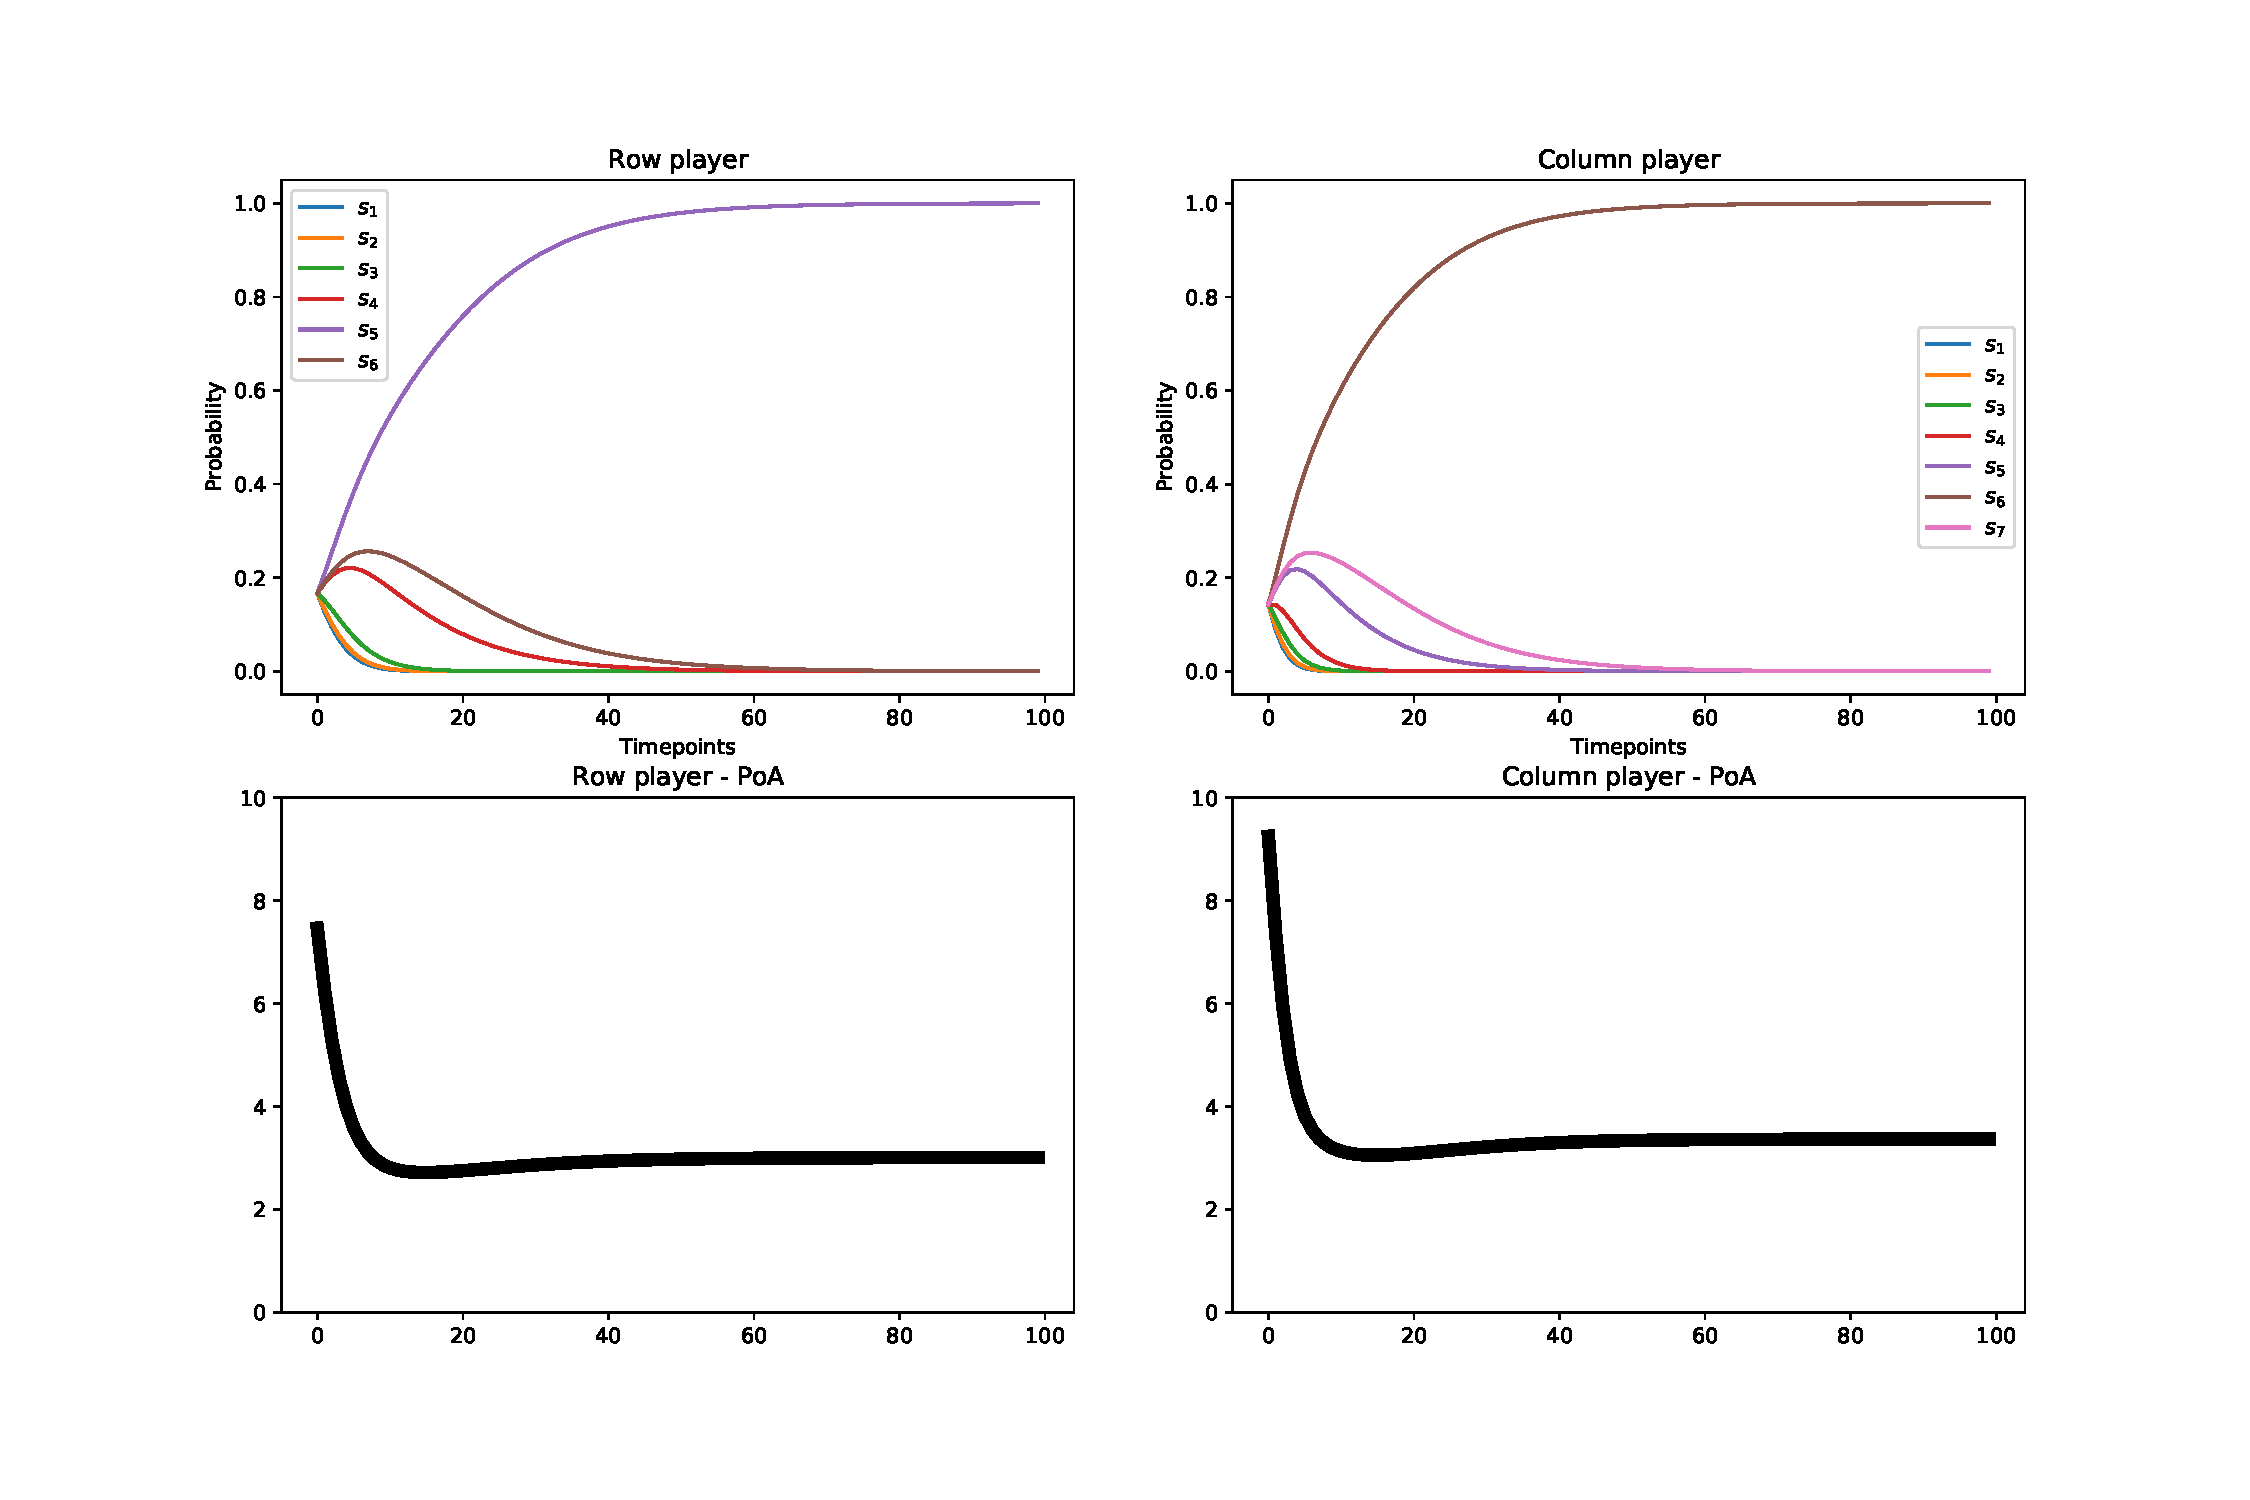
\includegraphics[width=\textwidth, trim=0 400 0 0]{imgs/asymmetric_rd_and_PoA/asymmetric_original.pdf}
    \caption{The strategies played when running asymmetric replicator dynamics
    along with the compartmentalised price of anarchy of the blocking time at
    each iteration of the learning algorithm}
    \label{fig:ard_original}
\end{figure}

It can be observed that the learning algorithm reaches a stable pair of 
strategies where \(T_1 = 5\) and \(T_2 = 6\). After a number of iterations the
price of anarchy for both players stabilises and barely increases until the 
final iteration. 

Figure \ref{fig:ard_lambda_2} shows a similar run of the
algorithm but when the strategies begin to stabilise a huge increase in the
arrival rate of ambulances occurs (i.e \( \lambda_2 = 10.7 \)).


\begin{figure}[H]
    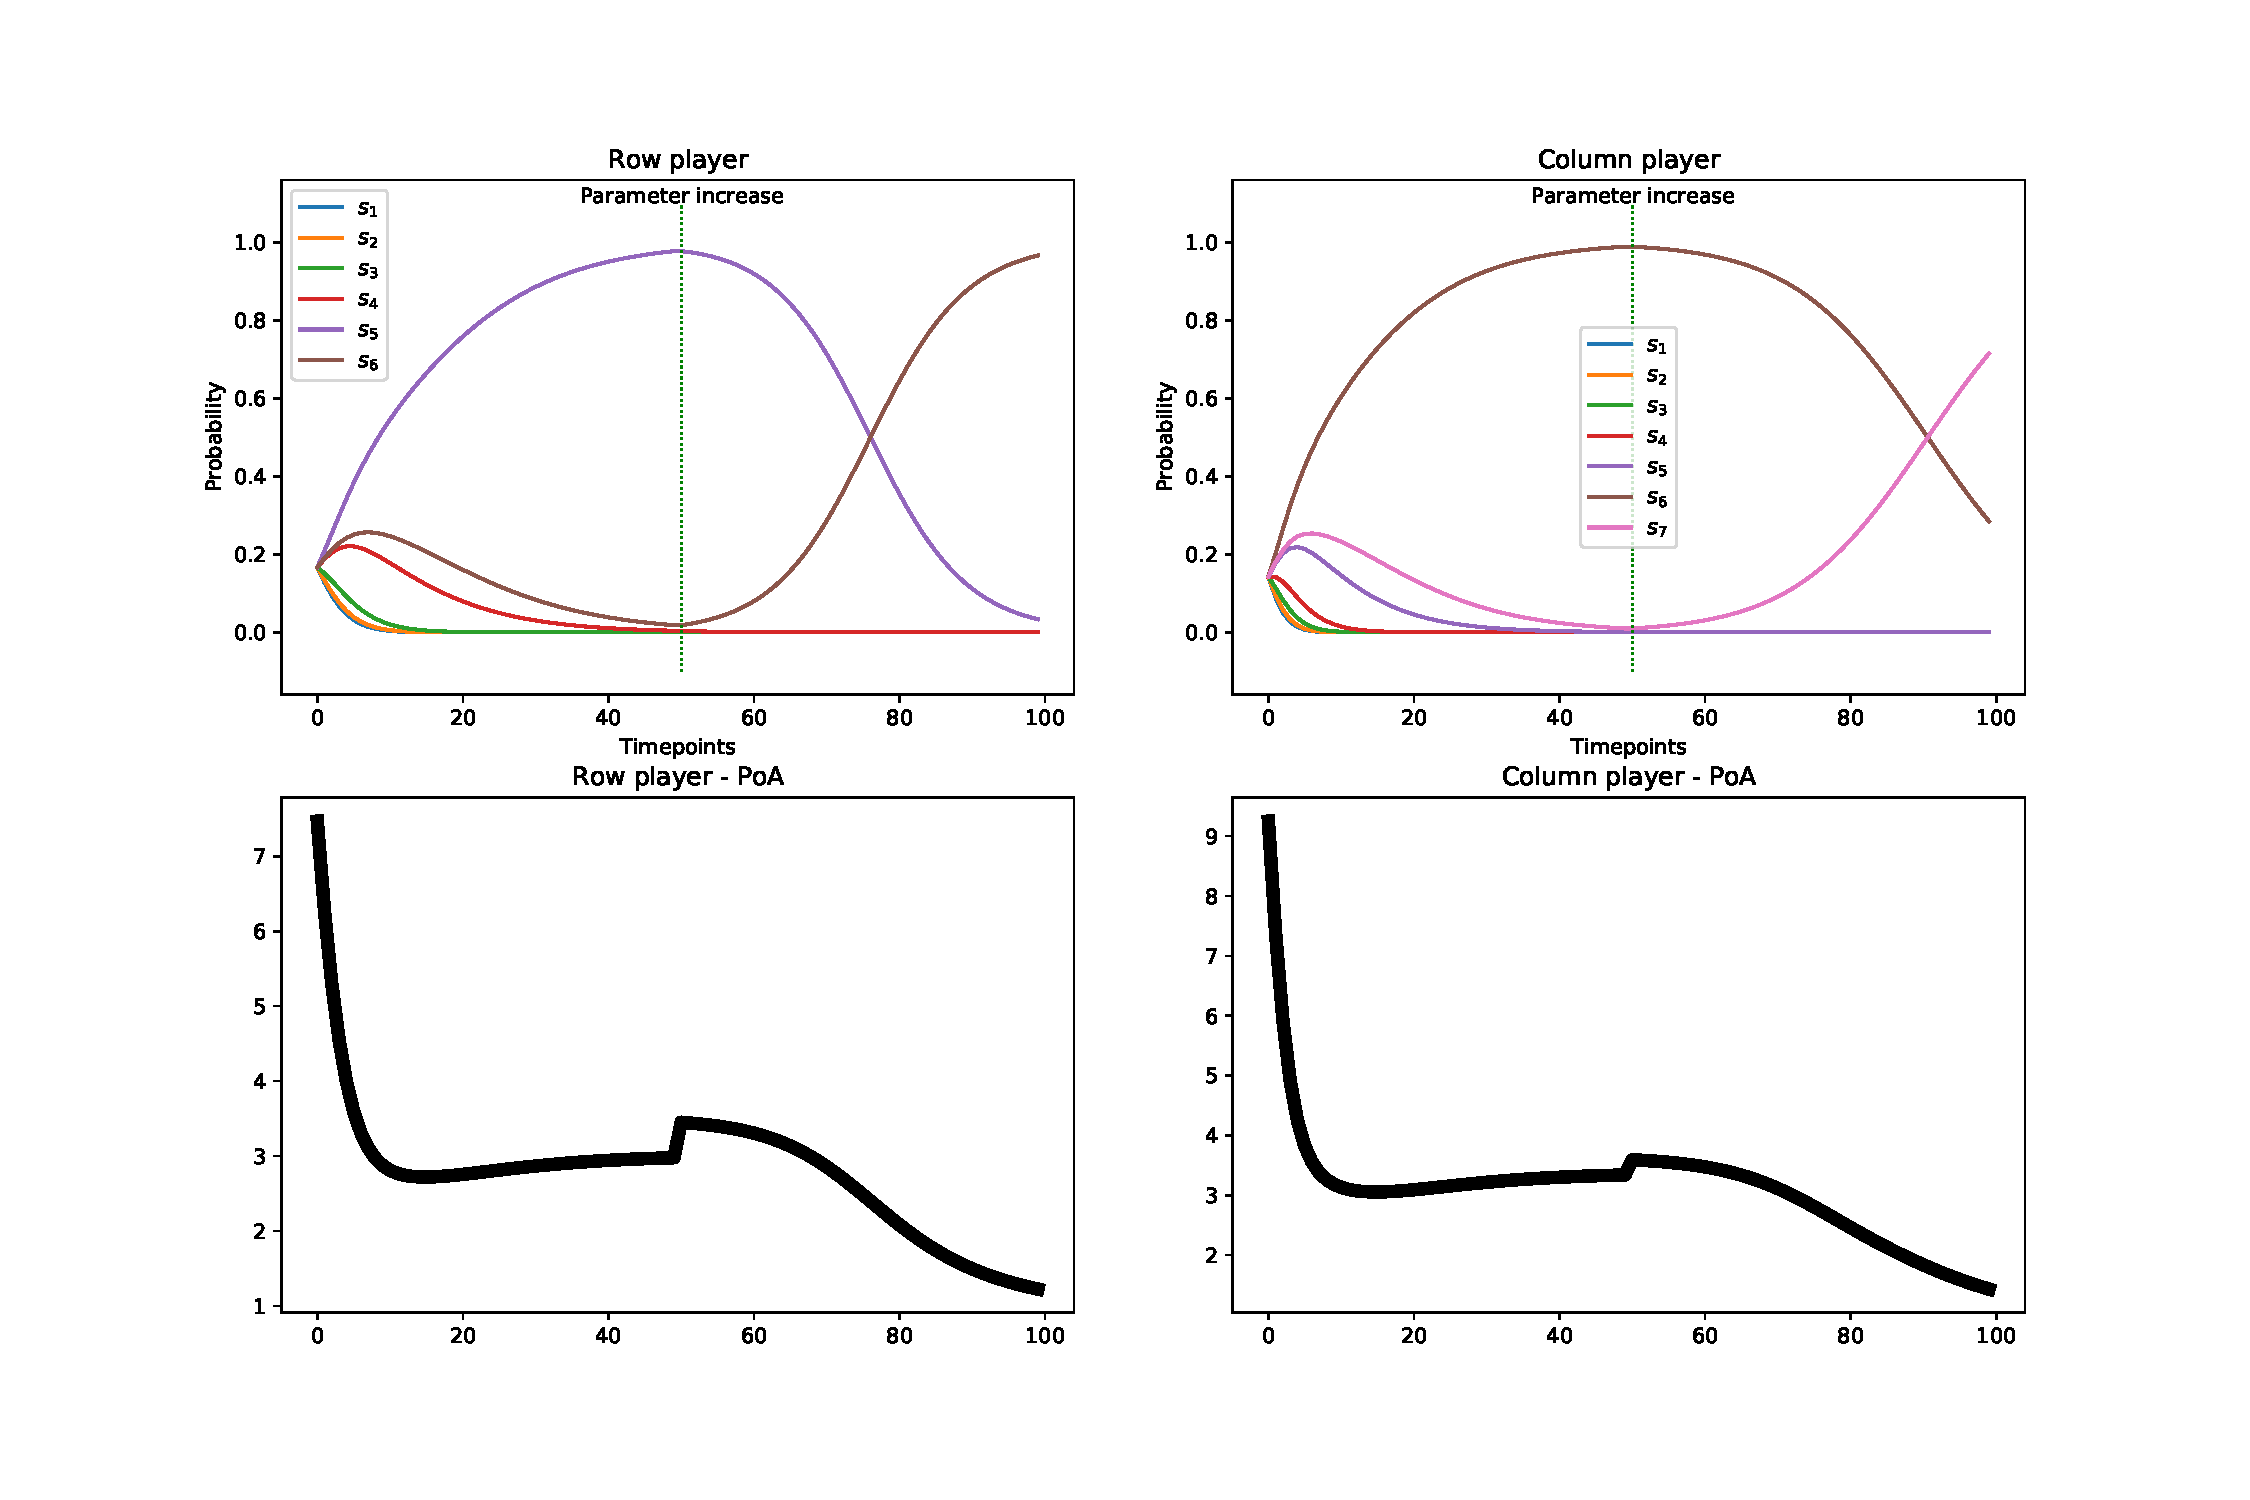
\includegraphics[width=\textwidth, trim=0 400 0 0]{imgs/asymmetric_rd_and_PoA/asymmetric_flooding.pdf}
    \caption{The strategies played when running asymmetric replicator dynamics
    along with the compartmentalised price of anarchy of the blocking time at
    each iteration of the learning algorithm. After a number of iterations the 
    arrival rate of ambulance patients is significantly increased to flood the
    system completely \( \lambda_2 = 10.7 \).}
    \label{fig:ard_lambda_2}
\end{figure}


By increasing \(\lambda_2\) there is no change in the how the players behave
(\(T_1 = 5, T_2 = 6\)), but the outcome of the system does change. 
There is a decline in the price of anarchy of the blocking time which at first 
glance indicates that upon flooding the system it becomes more efficient. 
This is non-sensical though.
What it really shows is that the steep increase in \( \lambda_2 \) simply leaves 
less potential for improvement. 

Figure \ref{fig:ard_num_of_servers} shows a run of asymmetric replicator 
dynamics with a change in the number of servers of both models.
The number of servers are increased from \(C_1 = 3, C_2 = 2\) to 
\(C_1 = 4, C_2 = 3\).


\begin{figure}[H]
    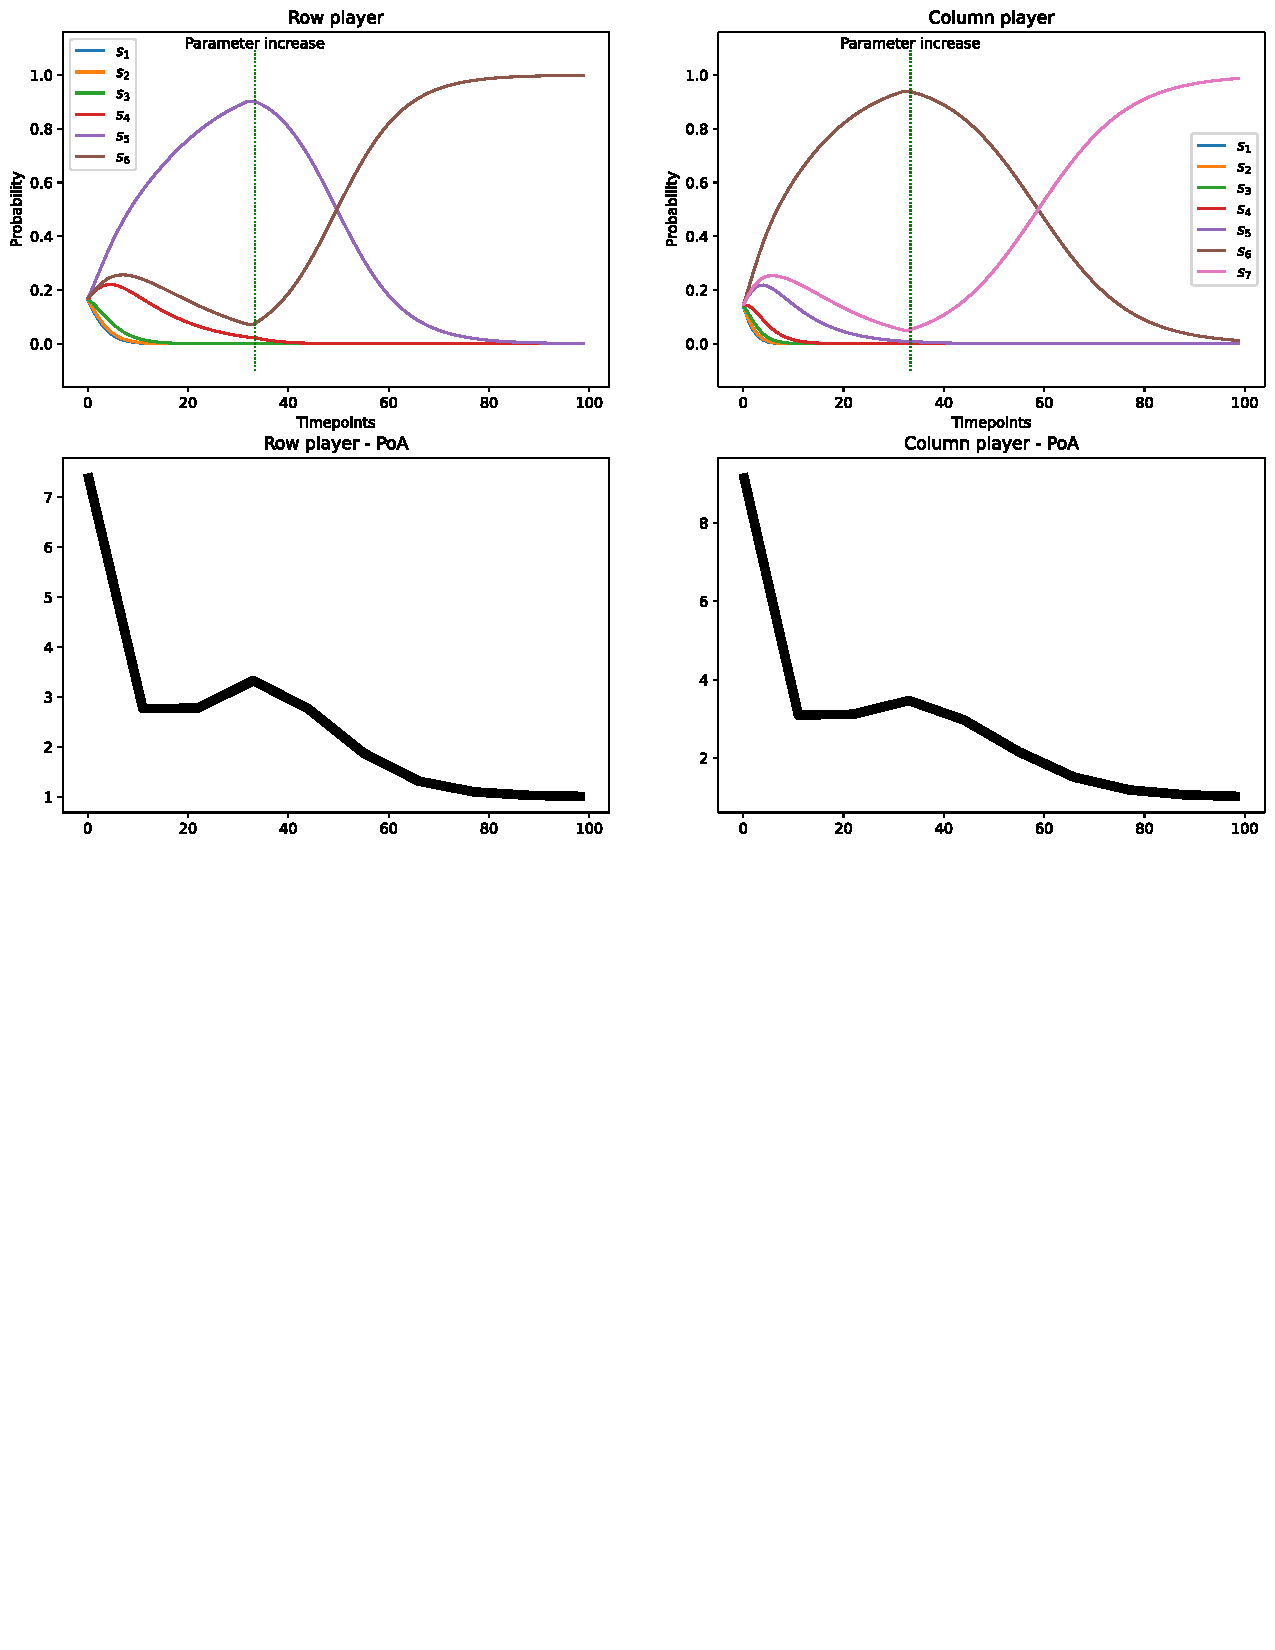
\includegraphics[width=\textwidth, trim=0 400 0 0]{imgs/asymmetric_rd_and_PoA/asymmetric_increase_C.pdf}
    \caption{
        The strategies played when running asymmetric replicator dynamics
        along with the compartmentalised price of anarchy of the blocking time 
        at each iteration of the learning algorithm. After a number of 
        iterations the number of servers for both systems are increased by one.
    }
    \label{fig:ard_num_of_servers}
\end{figure}

In this case the both the behaviour as well as the price of anarchy change.
The players change their strategies from \(T_1 = 5, T_2 = 6\) to 
\(T_1 = 6, T_2 = 7\) and the \(PoA\) of the blocking time goes down.
By adding more resources to the models they are able to increase their 
efficiency.
Although this is a good way to escape such inefficiencies, it might not always
be cost efficient.

Figure \ref{fig:ard_penalty} is slightly different than the previous ones.
Once asymmetric replicator dynamics becomes stable on some inefficient 
strategies (in terms of the blocking time) the payoff matrices of the two are
scaled in such a way so that the selected strategy is penalised.

\begin{figure}[H]
    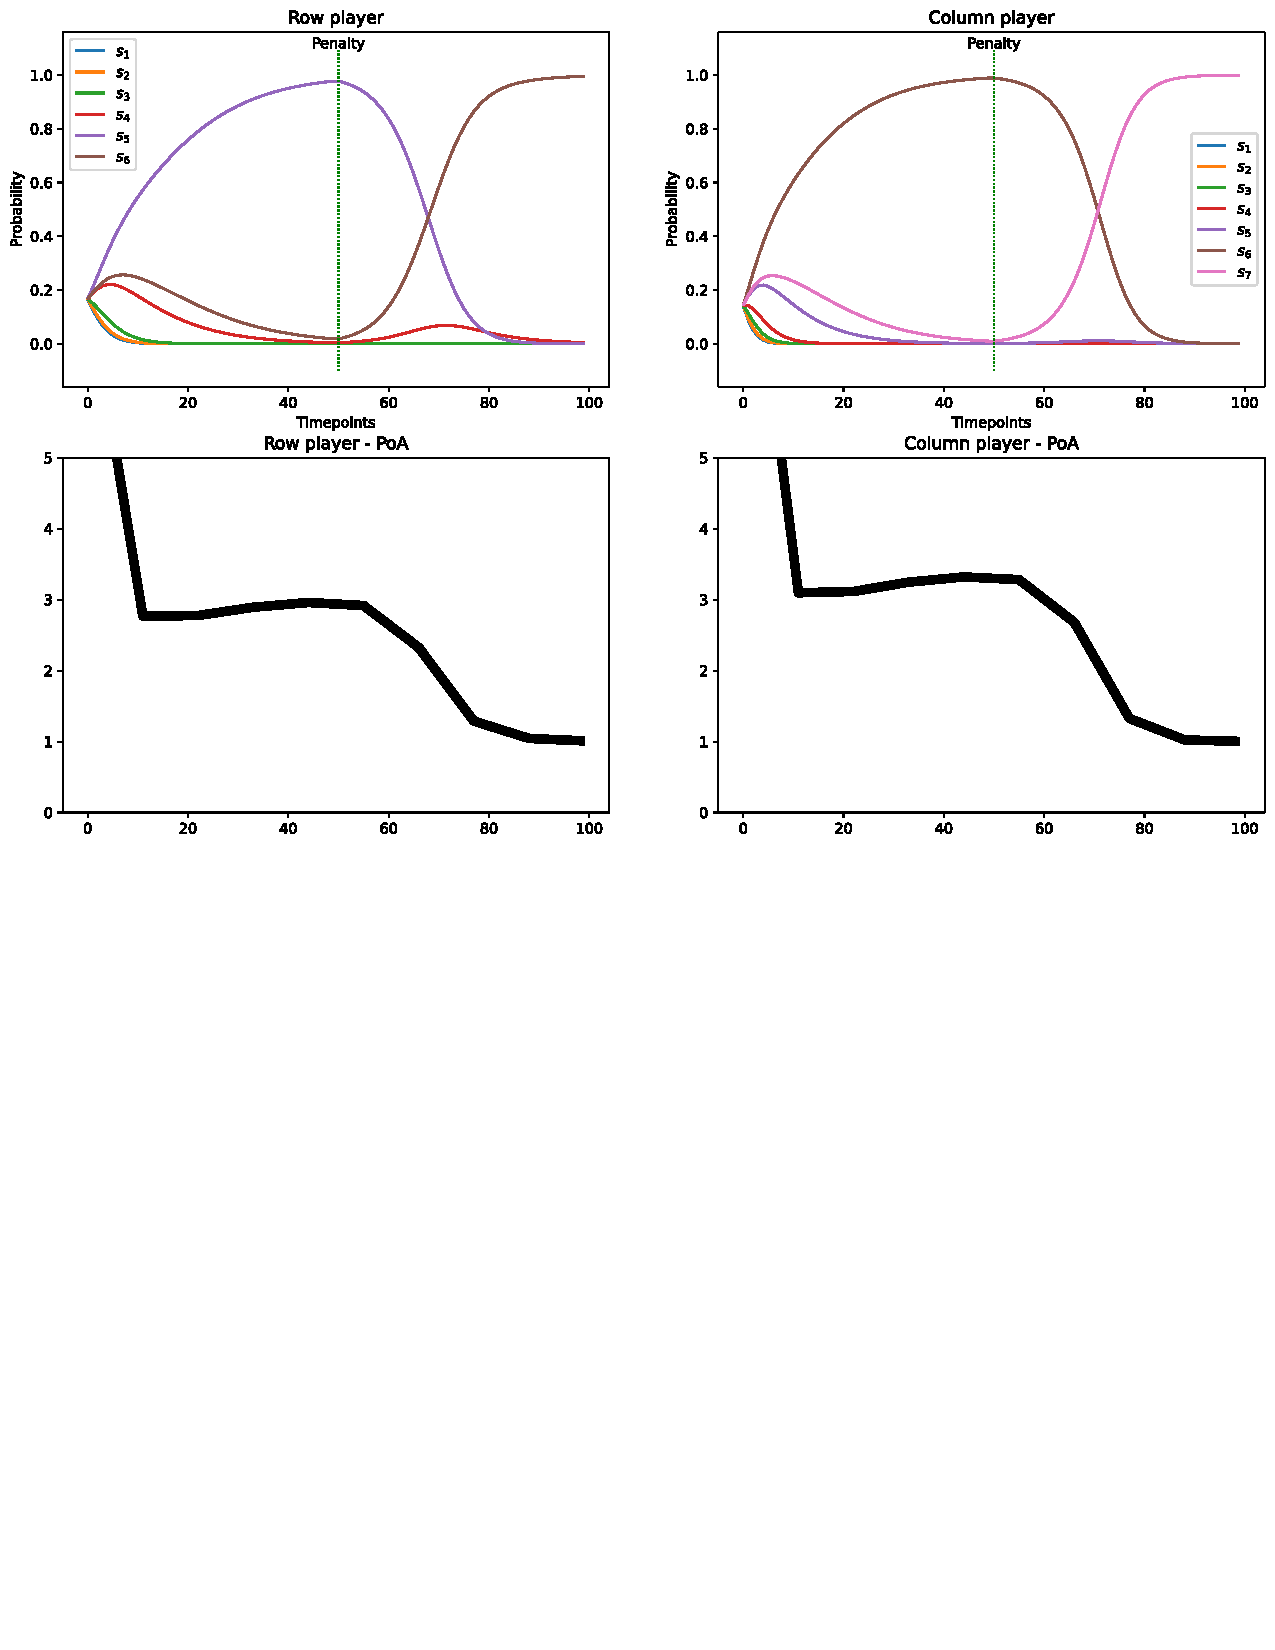
\includegraphics[width=\textwidth, trim=0 400 0 0]{imgs/asymmetric_rd_and_PoA/asymmetric_penalty.pdf}
    \caption{
        The strategies played when running asymmetric replicator dynamics
        along with the compartmentalised price of anarchy of the blocking time 
        at each iteration of the learning algorithm. After a number of 
        iterations the most dominant strategy is being penalised.
    }
    \label{fig:ard_penalty}
\end{figure}

By incentivising the players in such a way the players change their strategies 
and ambulance patients are accepted in the ED more often.
Thus the blocking time \(PoA\) for both EDs drops down. 

    \section{Conclusion}
    \newpage
    \bibliographystyle{plain}
    \bibliography{bibliography.bib}

    \begin{appendices}
    
    \section{Mean waiting time}\label{sec:appendix_mean_waiting}

The recursive formula described here is the origin of the closed-form formula 
described in section~\ref{sec:waiting_time}.

To calculate the mean waiting time one must first identify the set of states 
\((u, v)\) where a wait will occur. 
For this particular Markov chain, this points to all states that satisfy 
\(v > C\) i.e. all states where the number of individuals in the service centre 
exceed the number of servers. 
The set of such states is defined as \textit{waiting states} and can be denoted 
as a subset of all the states, where:

\begin{equation} \label{eq:waiting_states}
    S_w = \{(u, v) \in S \; | \; v > C \}    
\end{equation}

Additionally, there are certain states in the model where arrivals cannot occur. 
A type 1 individual cannot arrive whenever the model is at any state 
\((u, N)\) 
for all \(u\) where \(N\) is the system capacity. 
Equivalently, a type 2 individual cannot arrive in the model when the model is 
at any state \((M, v)\) for all \(v \geq T\).
Therefore the set of all such states that an arrival may occur are defined as 
\textit{accepting states} and are denoted as:

\begin{equation*}
    S_A^{(1)} = \{(u, v) \in S \; | \; v < N \}
    \tag{\ref{eq:accepting_states_type_1} revisited}
\end{equation*}

\begin{equation}
    S_A^{(2)}=
    \begin{cases}
        \{(u, v) \in S \; | \; u < M \} & \textbf{if } T \leq N\\
        \{(u, v) \in S \; | \; v < N \} & \textbf{otherwise}
    \end{cases}
    \tag{\ref{eq:accepting_states_type_2} revisited}
\end{equation}

Moreover, another element that needs to be considered is the expected waiting time 
% in each state \( c(u,v) \), otherwise known as sojourn time \cite{Raghunandanan}. 
In order to do so a variation of the Markov model has to be considered where when 
the individual arrives at any of the states of the model no more arrivals can 
occur after that. 


Thus, one may acquire the desired time by calculating the inverse of the sum of 
the out-flow rate of that state. 
Since arrivals are ignored though the only way to exit the state will only be 
via a service. 
In essence this notion can be expressed as:

\begin{equation} \label{eq:sojourn_type_1}
    c^{(1)}(u,v) = 
    \begin{cases}
        0, & \textbf{if } u > 0 \textbf{ and } v = T \\
        \frac{1}{\text{min}(v,C)\mu}, & \textbf{otherwise}
    \end{cases}
\end{equation}

Now, like in the type 1 individuals case, the sojourn time is needed. 
For type 2 individuals whenever individuals are at any row apart from the 
first one they automatically get a wait time of \(0\) since they are essentially 
blocked.

\begin{equation} \label{eq:sojourn_type_2}
    c^{(2)}(u,v) = 
    \begin{cases}
        0, & \textbf{if } u > 0 \\
        \frac{1}{\text{min}(v,C)\mu}, & \textbf{otherwise}
    \end{cases}
\end{equation}

Note that whenever any type 1 individual is at a state \((u,v)\) where 
\(u > 0\) 
and \(v = T\) (i.e. all states \((1,T), (2,T) \dots, (M,T)\)) the sojourn time is 
set to \(0\). 
This is done to capture the trip thorough the Markov chain from the perspective 
of individuals. 
Meaning that they will visit all states of the threshold column but only the one 
in the first row will return a non-zero sojourn time.
Thus, the expected waiting time of type 1 and type 2 individuals when upon
arriving at state \( (u,v) \) can be given by the following recursive formulas:

\begin{equation} \label{eq:waiting-time-at-each-state-type-1}
    w^{(1)}(u,v) = 
    \begin{cases} 
        0, \hspace{4.85cm} & \textbf{if } (u,v) \notin S_w \\
        c^{(1)}(u,v) + w^{(1)}(u-1, v), & \textbf{if } u > 0 \textbf{ and } v = T \\
        c^{(1)}(u,v) + w^{(1)}(u, v-1), & \textbf{otherwise}
    \end{cases}
\end{equation}

\begin{equation} \label{eq:waiting-time-at-each-state-type-2}
    w^{(2)}(u,v) = 
    \begin{cases} 
        0, \hspace{4.85cm} & \textbf{if } (u,v) \notin S_w \\
        c^{(2)}(u,v) + w^{(2)}(u-1, v), & \textbf{if } u > 0 \textbf{ and } v = T \\
        c^{(2)}(u,v) + w^{(2)}(u, v-1), & \textbf{otherwise}
    \end{cases}
\end{equation}

Finally, the mean waiting time can be calculated by summing over all expected 
waiting times of accepting states multiplied by the probability of being at that 
state and dividing by the probability of being in any accepting state.

\begin{equation} \label{eq:recursive-waiting-time-type-1}
    W^{(1)} = \frac{\sum_{(u,v) \in S_A^{(1)}} w^{(1)}(u,v) 
    \pi_{(u,v)}}{\sum_{(u,v) \in S_A^{(1)}} \pi_{(u,v)}}
\end{equation}

\begin{equation}\label{eq:recursive-waiting-time-type-2}
    W^{(2)} = \frac{\sum_{(u,v) \in S_A^{(2)}} w^{(2)}(u,v) \pi_{(u,v)}}
    {\sum_{(u,v) \in S_A^{(2)}} \pi_{(u,v)}}
\end{equation}

    \section{Mean blocking time} \label{sec:appendix_mean_blocking}

The set of states where individuals can be blocked is defined as:
\begin{equation*}
    S_b = \{(u,v) \in S \; | \; u > 0\} 
    \tag{\ref{eq:set_of_blocking_states} revisited}
\end{equation*}

The mean sojourn time for each state is given by the inverse of the out-flow of
that state ~\cite{Stewart2019}.
However, whenever a type 2 individual arrives at the system, no subsequent 
arrival of another type 2 individual can affect its pathway or total time in 
the system.
Therefore, looking at the mean time in the system from the perspective of an 
individual of the second type, all such type 2 arrivals need to be ignored.
Note here that this is not the case for individuals of the first type.
Whenever a type 2 individual is blocked and a type 1 individual arrives the type
2 individuals will stay blocked for some additional amount of time.
Thus, the mean time that a type 2 individual spends at each state is given by:

\begin{equation*}
    c(u,v) = 
    \begin{cases}
        \frac{1}{\min(v,C) \mu}, & \text{if } v = N\\
        \frac{1}{\lambda_1 + \min(v,C) \mu}, & \text{otherwise}
    \end{cases} 
    \tag{\ref{eq:sojourn_blocking_time} revisited}
\end{equation*}

In equation (\ref{eq:sojourn_blocking_time}), both service completions and 
type 1 arrivals are considered. 
Thus, from a blocked individual's perspective whenever the system moves from one 
state \((u,v)\)
to another state it can either:

\begin{itemize}
    \item be because of a service being completed: we will denote the probability 
    of this happening by \(p_s(u,v)\). 
    \item be because of an arrival of an individual of type 1: denoting such 
    probability by \(p_a(u,v)\).
\end{itemize}
The probabilities are given by:

\begin{equation*}
    p_s(u,v) = \frac{\min(v,C)\mu}{\lambda_1 + \min(v,C)\mu}, \qquad
    p_a(u,v) = \frac{\lambda_1}{\lambda_1 + \min(v,C)\mu}
    \tag{\ref{eq:probs_of_service_and_arrival} revisited} 
\end{equation*}


Having defined \(c(u,v)\) and \(S_b\) a formula for the blocking time that is
expected to occur at each state can be given by:

    \begin{equation*}
    b(u,v) = 
    \begin{cases} 
        0, & \textbf{if } (u,v) \notin S_b \\
        c(u,v) + b(u - 1, v), & \textbf{if } v = N = T\\
        c(u,v) + b(u, v-1), & \textbf{if } v = N \neq T \\
        c(u,v) + p_s(u,v) b(u-1, v) + p_a(u,v) b(u, v+1), & \textbf{if } u > 0 
        \textbf{ and } \vspace{-0.2cm} \\ 
        & \quad v = T \\
        c(u,v) + p_s(u,v) b(u, v-1) + p_a(u,v) b(u, v+1), & \textbf{otherwise} \\
    \end{cases}
    \tag{\ref{eq:general_blocking_time_at_each_state} revisited}
\end{equation*}

A direct approach will be used to solve this equation here. 
By enumerating all equations of (\ref{eq:general_blocking_time_at_each_state}) 
for all states \((u,v)\) that belong in \(S_b\) 
a system of linear equations arises where the unknown variables are all the 
\(b(u,v)\) terms. 
Note here that these equations correspond to all blocking states as defined in
(\ref{eq:set_of_blocking_states}). 
Equations that correspond to non-blocking states have a value of \(0\) as 
defined in (\ref{eq:general_blocking_time_at_each_state})
The general form of the equation in terms of \(C,T,N \text{ and } M\) is given by: 

\begin{align}
    b(1,T) \quad &= \quad c(1, T) + p_a b(1, T + 1) \label{eq:first_eq_of_blocking_general}\\
    b(1,T + 1) \quad &= \quad c(1, T + 1) + p_s b(1, T) + p_a b(1, T + 1) \\
    b(1,T + 2) \quad &= \quad c(1, T + 2) + p_s b(1, T + 1) + p_a b(1, T + 3) \\
    & \ \, \vdots \nonumber \\
    b(1, N) \quad &= \quad c(1, N) + b(1, N - 1) \\
    b(2, T) \quad &= \quad c(2, T) + p_s b(1, T) + p_a b(2, T + 1) \\
    b(2, T + 1) \quad &= \quad c(2, T + 1) + p_s b(2, T) + p_a b(2, T + 2) \\
    & \ \, \vdots \nonumber \\
    b(M - 1, N) \quad &= \quad c(M, N - 1) + b(M, N-1) \\ 
    b(M, T) \quad &= \quad c(T, N) + p_s b(T-1, N) + p_a b(T, N+1) \\
    & \ \, \vdots \nonumber \\
    b(M, N) \quad &= \quad c(M, N) + b(M, N-1) \label{eq:last_eq_of_blocking_general}
\end{align}

The equivalent matrix notation of the linear system of equations 
(\ref{eq:first_eq_of_blocking_general}) - (\ref{eq:last_eq_of_blocking_general})
is given by \(Zx=y\), where:
\begin{equation}
    \scalebox{0.73}{\(
        Z = 
        \begin{pmatrix}
            -1 & p_a & 0 & \dots & 0 & 0 & 0 & 0 & 0 & \dots & 0 & 0 \\ %(1,T)
            p_s & -1 & p_a & \dots & 0 & 0 & 0 & 0 & 0 & \dots & 0 & 0 \\ %(1,T+1)
            0 & p_s & -1 & \dots & 0 & 0 & 0 & 0 & 0 & \dots & 0 & 0 \\ %(1,T+2)
            \vdots & \vdots & \vdots & \ddots & \vdots & \vdots & \vdots & 
            \vdots & \vdots & \ddots & \vdots & \vdots \\ 
            0 & 0 & 0 & \dots & 1 & -1 & 0 & 0 & 0 & \dots & 0 & 0 \\ %(1,N)
            p_s & 0 & 0 & \dots & 0 & 0 & -1 & p_a & 0 & \dots & 0 & 0 \\ %(2,T)
            0 & 0 & 0 & \dots & 0 & 0 & p_s & -1 & p_a & \dots & 0 & 0 \\ %(2,T+1)
            \vdots & \vdots & \vdots & \ddots & \vdots & \vdots & \vdots & 
            \vdots & \vdots & \ddots & \vdots & \vdots \\ 
            0 & 0 & 0 & \dots & 0 & 0 & 0 & 0 & 0 & \dots & 1 & -1 \\ %(M,N)
        \end{pmatrix},
        x = 
        \begin{pmatrix}
            b(1,T) \\
            b(1,T+1) \\
            b(1,T+2) \\
            \vdots \\
            b(1,N) \\
            b(2,T) \\
            b(2,T+1) \\
            \vdots \\
            b(M,N) \\
        \end{pmatrix}, 
        y= 
        \begin{pmatrix}
            -c(1,T) \\
            -c(1,T+1) \\
            -c(1,T+2) \\
            \vdots \\
            -c(1,N) \\
            -c(2,T) \\
            -c(2,T+1) \\
            \vdots \\
            -c(M,N) \\
        \end{pmatrix}
    \)} \tag{\ref{eq:general_algebaric_approach_blocking_time} revisited}
    \end{equation}

    The elements of the matrix \(Z\) can be acquired using \(Z_{ij}\) defined in 
    equation (\ref{eq:general_mapping_function_of_blocking_matrix}) where \(i\) 
    and \(j\) are states \((u_i, v_i), (u_j, v_j) \in S_b\) 
    (\ref{eq:set_of_blocking_states}).

    \begin{equation}
    Z_{ij} = 
    \begin{cases}
        p_a, & \textbf{if } j = i + 1 \textbf{ and } v_i \neq N \\
        p_s, & \textbf{if } j = i - 1 \textbf{ and } v_i \neq N, v_i \neq T \\
            & \textbf{or } j = i - N + T \textbf{ and } u_i \geq 2,\,v_i = T \\
        1, & \textbf{if } j = i - 1 \textbf{ and } v_i = N \\
        -1, & \textbf{if } i = j \\
        0, & \textbf{otherwise} \\
    \end{cases}
    \tag{\ref{eq:general_mapping_function_of_blocking_matrix} revisited}
\end{equation}


Thus, having calculated the mean blocking time for all blocking states 
\(b(u,v)\), they can be combined together in a formula.
The resultant formula for the mean blocking time is given by:

\begin{equation}
    B = \frac{\sum_{(u,v) \in S_A} \pi_{(u,v)} \; b(u,v)}{\sum_{(u,v) \in S_A} 
    \pi_{(u,v)}} \tag{\ref{eq:algebraic_blocking_time} revisited}
\end{equation}

To illustrate how the described formula works consider a Markov model where 
\(C=2, T=2, N=4, M=2\) (figure \ref{fig:example_algeb_blocking}). 
The equations that correspond to such a model are shown in 
(\ref{eq:first_eq_of_blocking_example})-(\ref{eq:last_eq_of_blocking_example}) 
and their equivalent matrix notation form is shown in 
(\ref{eq:example_algebaric_approach_blocking_time}).

\begin{minipage}{.5\textwidth}
    \begin{figure}[H]
        \scalebox{0.6}{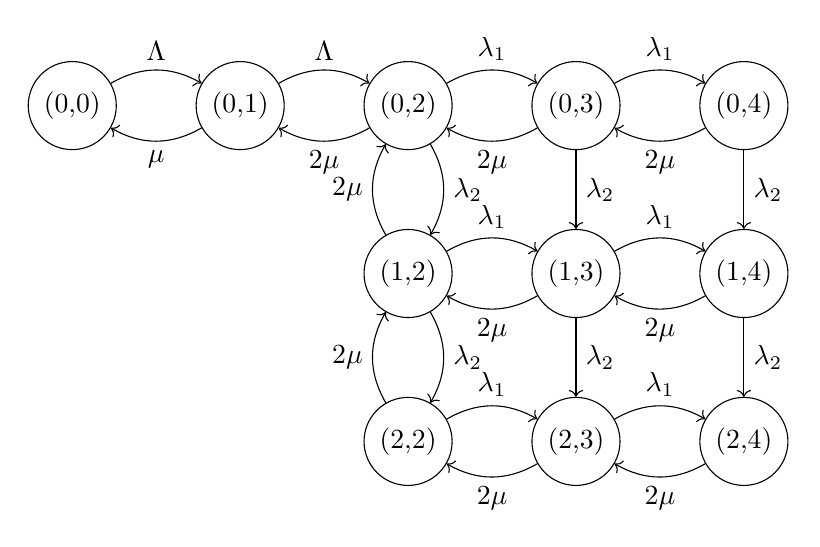
\begin{tikzpicture}[-, node distance = 1cm, auto]
\node[state] (u0v0) {(0,0)};
\node[state, right=of u0v0] (u0v1) {(0,1)};
\draw[->](u0v0) edge[bend left] node {\( \Lambda \)} (u0v1);
\draw[->](u0v1) edge[bend left] node {\(\mu \)} (u0v0);
\node[state, right=of u0v1] (u0v2) {(0,2)};
\draw[->](u0v1) edge[bend left] node {\( \Lambda \)} (u0v2);
\draw[->](u0v2) edge[bend left] node {\(2\mu \)} (u0v1);
\node[state, below=of u0v2] (u1v2) {(1,2)};
\draw[->](u0v2) edge[bend left] node {\( \lambda_2 \)} (u1v2);
\draw[->](u1v2) edge[bend left] node {\(2\mu \)} (u0v2);
\node[state, below=of u1v2] (u2v2) {(2,2)};
\draw[->](u1v2) edge[bend left] node {\( \lambda_2 \)} (u2v2);
\draw[->](u2v2) edge[bend left] node {\(2\mu \)} (u1v2);
\node[state, right=of u0v2] (u0v3) {(0,3)};
\draw[->](u0v2) edge[bend left] node {\( \lambda_1 \)} (u0v3);
\draw[->](u0v3) edge[bend left] node {\(2\mu \)} (u0v2);
\node[state, right=of u1v2] (u1v3) {(1,3)};
\draw[->](u1v2) edge[bend left] node {\( \lambda_1 \)} (u1v3);
\draw[->](u1v3) edge[bend left] node {\(2\mu \)} (u1v2);
\draw[->](u0v3) edge node {\( \lambda_2 \)} (u1v3);
\node[state, right=of u2v2] (u2v3) {(2,3)};
\draw[->](u2v2) edge[bend left] node {\( \lambda_1 \)} (u2v3);
\draw[->](u2v3) edge[bend left] node {\(2\mu \)} (u2v2);
\draw[->](u1v3) edge node {\( \lambda_2 \)} (u2v3);
\node[state, right=of u0v3] (u0v4) {(0,4)};
\draw[->](u0v3) edge[bend left] node {\( \lambda_1 \)} (u0v4);
\draw[->](u0v4) edge[bend left] node {\(2\mu \)} (u0v3);
\node[state, right=of u1v3] (u1v4) {(1,4)};
\draw[->](u1v3) edge[bend left] node {\( \lambda_1 \)} (u1v4);
\draw[->](u1v4) edge[bend left] node {\(2\mu \)} (u1v3);
\draw[->](u0v4) edge node {\( \lambda_2 \)} (u1v4);
\node[state, right=of u2v3] (u2v4) {(2,4)};
\draw[->](u2v3) edge[bend left] node {\( \lambda_1 \)} (u2v4);
\draw[->](u2v4) edge[bend left] node {\(2\mu \)} (u2v3);
\draw[->](u1v4) edge node {\( \lambda_2 \)} (u2v4);
\end{tikzpicture}}
        \caption{
            \centering{Example of Markov chain with \(C=2, T=2, N=4, M=2\)}
        }
        \label{fig:example_algeb_blocking}
    \end{figure}
    \end{minipage}
    \begin{minipage}{.43\textwidth}
    \begin{align}
        b(1,2) &= c(1,2) + p_a b(1,3) \label{eq:first_eq_of_blocking_example} \\
        b(1,3) &= c(1,3) + p_s b(1,2) \nonumber \\ &+ p_a b(1,4) \\
        b(1,4) &= c(1,4) + b(1,3) \\
        b(2,2) &= c(2,2) + p_s b(1,2) \nonumber \\ &+ p_a b(2,3) \\
        b(2,3) &= c(2,3) + p_s b(2,2) \nonumber \\ &+ p_a b(1,4) \\
        b(2,4) &= c(2,4) + b(2,3) \label{eq:last_eq_of_blocking_example}
    \end{align}
\end{minipage}

\begin{equation}\label{eq:example_algebaric_approach_blocking_time}
    Z=
    \begin{pmatrix}
        -1 & p_a & 0 & 0 & 0 & 0 \\ %(1,2)
        p_s & -1 & p_a & 0 & 0 & 0 \\ %(1,3)
        0 & 1 & -1 & 0 & 0 & 0 \\ %(1,4)
        p_s & 0 & 0 & -1 & p_a & 0\\ %(2,2)
        0 & 0 & 0 & p_s & -1 & p_a \\ %(2,3)
        0 & 0 & 0 & 0 & 1 & -1 \\ %(2,4)
    \end{pmatrix},
    x=
    \begin{pmatrix}
        b(1,2) \\
        b(1,3) \\
        b(1,4) \\
        b(2,2) \\
        b(2,3) \\
        b(2,4) \\
    \end{pmatrix}, 
    y=
    \begin{pmatrix}
        -c(1,2) \\
        -c(1,3) \\
        -c(1,4) \\
        -c(2,2) \\
        -c(2,3) \\
        -c(2,4) \\
    \end{pmatrix}
\end{equation}

    \section{Mean blocking time} \label{sec:appendix_mean_proportion}
    
In order to consider such measure though one would need to obtain the 
distribution of time in the system for all individuals. 
The complexity of such task is caused by the fact that different individuals 
arrive at different states of the Markov model. 
Consider the case when an arrival occurs when the model is at a specific state.

\paragraph{Time distribution at specific state (1 server):}

\begin{figure}[H]
    \centering
    \scalebox{0.75}{
        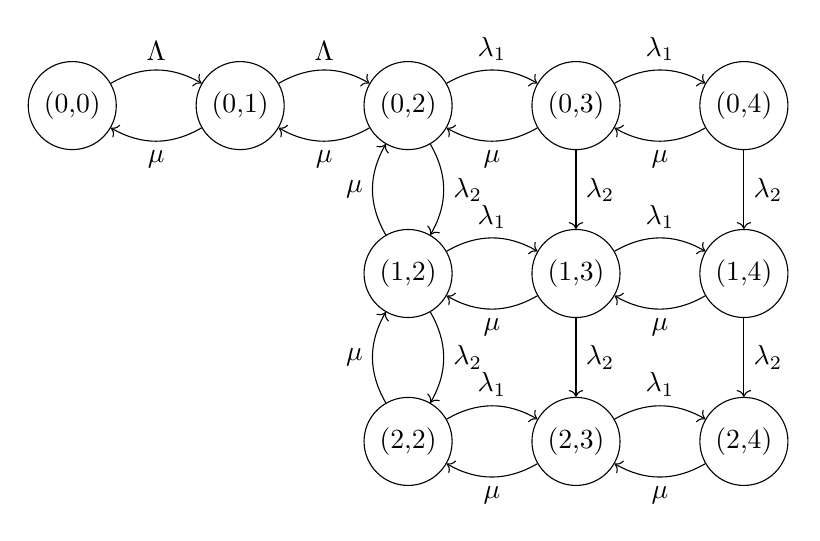
\begin{tikzpicture}[-, node distance = 1cm, auto]
\node[state] (u0v0) {(0,0)};
\node[state, right=of u0v0] (u0v1) {(0,1)};
\draw[->](u0v0) edge[bend left] node {\( \Lambda \)} (u0v1);
\draw[->](u0v1) edge[bend left] node {\(\mu \)} (u0v0);
\node[state, right=of u0v1] (u0v2) {(0,2)};
\draw[->](u0v1) edge[bend left] node {\( \Lambda \)} (u0v2);
\draw[->](u0v2) edge[bend left] node {\(\mu \)} (u0v1);
\node[state, below=of u0v2] (u1v2) {(1,2)};
\draw[->](u0v2) edge[bend left] node {\( \lambda_2 \)} (u1v2);
\draw[->](u1v2) edge[bend left] node {\(\mu \)} (u0v2);
\node[state, below=of u1v2] (u2v2) {(2,2)};
\draw[->](u1v2) edge[bend left] node {\( \lambda_2 \)} (u2v2);
\draw[->](u2v2) edge[bend left] node {\(\mu \)} (u1v2);
\node[state, right=of u0v2] (u0v3) {(0,3)};
\draw[->](u0v2) edge[bend left] node {\( \lambda_1 \)} (u0v3);
\draw[->](u0v3) edge[bend left] node {\(\mu \)} (u0v2);
\node[state, right=of u1v2] (u1v3) {(1,3)};
\draw[->](u1v2) edge[bend left] node {\( \lambda_1 \)} (u1v3);
\draw[->](u1v3) edge[bend left] node {\(\mu \)} (u1v2);
\draw[->](u0v3) edge node {\( \lambda_2 \)} (u1v3);
\node[state, right=of u2v2] (u2v3) {(2,3)};
\draw[->](u2v2) edge[bend left] node {\( \lambda_1 \)} (u2v3);
\draw[->](u2v3) edge[bend left] node {\(\mu \)} (u2v2);
\draw[->](u1v3) edge node {\( \lambda_2 \)} (u2v3);
\node[state, right=of u0v3] (u0v4) {(0,4)};
\draw[->](u0v3) edge[bend left] node {\( \lambda_1 \)} (u0v4);
\draw[->](u0v4) edge[bend left] node {\(\mu \)} (u0v3);
\node[state, right=of u1v3] (u1v4) {(1,4)};
\draw[->](u1v3) edge[bend left] node {\( \lambda_1 \)} (u1v4);
\draw[->](u1v4) edge[bend left] node {\(\mu \)} (u1v3);
\draw[->](u0v4) edge node {\( \lambda_2 \)} (u1v4);
\node[state, right=of u2v3] (u2v4) {(2,4)};
\draw[->](u2v3) edge[bend left] node {\( \lambda_1 \)} (u2v4);
\draw[->](u2v4) edge[bend left] node {\(\mu \)} (u2v3);
\draw[->](u1v4) edge node {\( \lambda_2 \)} (u2v4);
\end{tikzpicture}
    }
    \caption{Example Markov model \(C=1, T=2, N=4, M=2\)}
    \label{fig:distribution_of_time_at_specific_state_1_server}
\end{figure}

Consider the Markov model of figure 
\ref{fig:distribution_of_time_at_specific_state_1_server} with one server and a 
threshold of two individuals. 
Assume that an individual of the first type arrives when the model is at state 
\((0,3)\), thus forcing the model to move to state \((0,4)\). 
The distribution of the time needed for the specified individual to exit the 
system from state \((0,4)\) is given by the sum of exponentially distributed 
random variables with the same parameter \(\mu\). 
The sum of such random variables forms an Erlang distribution which is defined 
by the number of random variables that are added and their exponential 
parameter.
Note here that these random variables represent the individual's pathway from 
the perspective of the individual. 
Thus, \(X_i\) represents the time that it takes to move from the 
\(i^{\text{th}}\) position of the queue to the \((i-1)^{\text{th}}\) position 
(i.e. for someone in front of them to finish their service) and \(X_0\) is the 
time it takes to move from having a service to exiting the system.

\begin{align}
    (0,4) \Rightarrow \quad & X_3 \sim Exp(\mu) \nonumber \\
    (0,3) \Rightarrow \quad & X_2 \sim Exp(\mu) \nonumber \\
    (0,2) \Rightarrow \quad & X_1 \sim Exp(\mu) \nonumber \\
    (0,1) \Rightarrow \quad & X_0 \sim Exp(\mu) \nonumber \\
    S = X_3 + X_2 + & X_1 + X_0 = Erlang(4, \mu)
\end{align}

Thus, the waiting and service time of an individual in the model of figure 
\ref{fig:distribution_of_time_at_specific_state_1_server} can be captured by an 
erlang distributed random variable. 
The general CDF of the erlang distribution \(Erlang(k, \mu)\) is given by:

\begin{equation} \label{eq:cdf_erlang}
    P(S < t) = 1 - \sum_{i=0}^{k-1} \frac{1}{i!} e^{-\mu t} (\mu t)^i
\end{equation}

Unfortunately, the erlang distribution can only be used for the sum of 
identically distributed random variables from the exponential distribution. 
Therefore, this approach cannot be used when one of the random variables has a 
different parameter than the others. 
In fact the only case where it can be used is only when the number of servers 
are \(C=1\), or when an individual arrives and goes straight to service 
(i.e. when there is no other individual waiting and there is an empty server).


\paragraph{Time distribution at a state (multiple servers):}

\begin{figure}[H]
    \centering
    \scalebox{0.75}{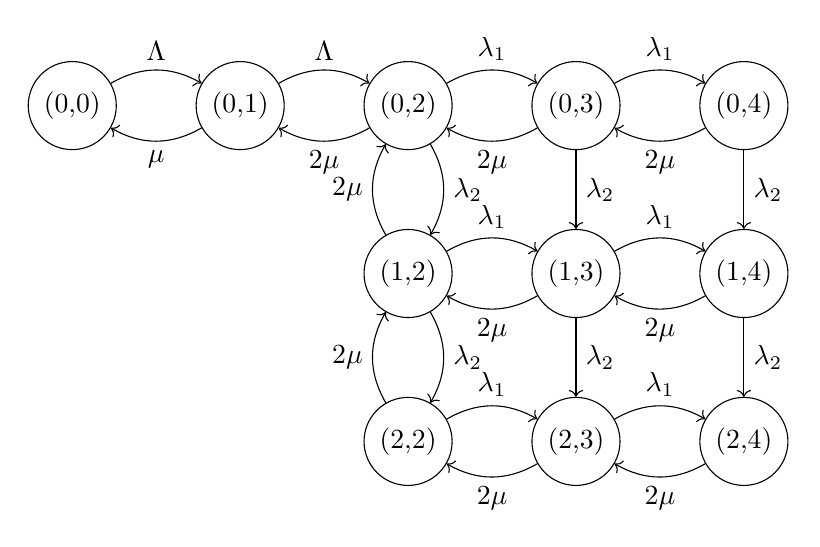
\begin{tikzpicture}[-, node distance = 1cm, auto]
\node[state] (u0v0) {(0,0)};
\node[state, right=of u0v0] (u0v1) {(0,1)};
\draw[->](u0v0) edge[bend left] node {\( \Lambda \)} (u0v1);
\draw[->](u0v1) edge[bend left] node {\(\mu \)} (u0v0);
\node[state, right=of u0v1] (u0v2) {(0,2)};
\draw[->](u0v1) edge[bend left] node {\( \Lambda \)} (u0v2);
\draw[->](u0v2) edge[bend left] node {\(2\mu \)} (u0v1);
\node[state, below=of u0v2] (u1v2) {(1,2)};
\draw[->](u0v2) edge[bend left] node {\( \lambda_2 \)} (u1v2);
\draw[->](u1v2) edge[bend left] node {\(2\mu \)} (u0v2);
\node[state, below=of u1v2] (u2v2) {(2,2)};
\draw[->](u1v2) edge[bend left] node {\( \lambda_2 \)} (u2v2);
\draw[->](u2v2) edge[bend left] node {\(2\mu \)} (u1v2);
\node[state, right=of u0v2] (u0v3) {(0,3)};
\draw[->](u0v2) edge[bend left] node {\( \lambda_1 \)} (u0v3);
\draw[->](u0v3) edge[bend left] node {\(2\mu \)} (u0v2);
\node[state, right=of u1v2] (u1v3) {(1,3)};
\draw[->](u1v2) edge[bend left] node {\( \lambda_1 \)} (u1v3);
\draw[->](u1v3) edge[bend left] node {\(2\mu \)} (u1v2);
\draw[->](u0v3) edge node {\( \lambda_2 \)} (u1v3);
\node[state, right=of u2v2] (u2v3) {(2,3)};
\draw[->](u2v2) edge[bend left] node {\( \lambda_1 \)} (u2v3);
\draw[->](u2v3) edge[bend left] node {\(2\mu \)} (u2v2);
\draw[->](u1v3) edge node {\( \lambda_2 \)} (u2v3);
\node[state, right=of u0v3] (u0v4) {(0,4)};
\draw[->](u0v3) edge[bend left] node {\( \lambda_1 \)} (u0v4);
\draw[->](u0v4) edge[bend left] node {\(2\mu \)} (u0v3);
\node[state, right=of u1v3] (u1v4) {(1,4)};
\draw[->](u1v3) edge[bend left] node {\( \lambda_1 \)} (u1v4);
\draw[->](u1v4) edge[bend left] node {\(2\mu \)} (u1v3);
\draw[->](u0v4) edge node {\( \lambda_2 \)} (u1v4);
\node[state, right=of u2v3] (u2v4) {(2,4)};
\draw[->](u2v3) edge[bend left] node {\( \lambda_1 \)} (u2v4);
\draw[->](u2v4) edge[bend left] node {\(2\mu \)} (u2v3);
\draw[->](u1v4) edge node {\( \lambda_2 \)} (u2v4);
\end{tikzpicture}}
    \caption{Example Markov model \(C=2, T=2, N=4, M=2\)}
    \label{fig:distribution_of_time_at_specific_state_2_servers}
\end{figure}

Figure \ref{fig:distribution_of_time_at_specific_state_2_servers} represents the 
same Markov model as figure 
\ref{fig:distribution_of_time_at_specific_state_1_server} with the only 
exception that there are 2 servers here. 
By applying the same logic, assuming that an individual arrives at state 
\((0,4)\), the sum of the following random variables arises.

\begin{align}
    (0,4) \Rightarrow \quad & X_2 \sim Exp(2\mu) \nonumber \\
    (0,3) \Rightarrow \quad & X_1 \sim Exp(2\mu) \\
    (0,2) \Rightarrow \quad & X_0 \sim Exp(\mu) \nonumber
\end{align}

Since these exponentially distributed random variables do not share the same 
parameter, an erlang distribution cannot be used. 
In fact, the problem can now be viewed either as the sum of exponentially 
distributed random variables with different parameters or as the sum of 
erlang distributed random variables.
The sum of erlang distributed random variables is said to follow the 
hypoexponential distribution. 
The hypoexponential distribution is defined with two vectors of size equal
to the number of Erlang random variables \cite{Akkouchi2008}, \cite{Smaili2013}. 
The vector \(\vec{r}\) contains all the \(k\)-values of the erlang distributions 
and \(\vec{\lambda}\) is a vector of the distinct parameters as illustrated in
equation (\ref{eq:connection_between_Hypoexponential_Erlang}).

\begin{equation}\label{eq:connection_between_Hypoexponential_Erlang}
    \begin{rcases}
        Erlang(k_1, \lambda_1) \\
        Erlang(k_2, \lambda_2) \\
        \hspace{1cm} \vdots \\
        Erlang(k_n, \lambda_n)
    \end{rcases}
    Hypo(
        \underbrace{(k_1, k_2, \dots k_n)}_{\vec{k}}, 
        \underbrace{(\lambda_1, \lambda_2, \dots \lambda_n)}_{\vec{\lambda}}
    )
\end{equation}

Equivalently, for this particular example:
\begin{align} \label{eq:multiple_servers_distribution_example}
    \begin{rcases}
        \begin{rcases}
            \scriptstyle{X_2 \sim Exp(2\mu)} \\
            \scriptstyle{X_1 \sim Exp(2\mu)}
        \end{rcases}
        \scriptstyle{X_1 + X_2 = S_1 \sim Erlang(2, 2\mu)} \\
        \scriptstyle{X_0 \sim Exp(\mu) \Rightarrow 
        \hspace{1cm} X_0 = S_2 \sim Erlang(1, \mu)}
    \end{rcases}
    \scriptstyle{S_1 + S_2 = H \sim Hypo((2,1), (2\mu, \mu))}
\end{align}

Therefore, the CDF of this distribution can be used to get the probability of 
the time in spent in the system being less than a given target.
The general CDF of the hypoexponential distribution \(Hypo(\vec{r}, 
\vec{\lambda})\), is given by the following expression \cite{Favaro2010}:

\begin{align} \label{eq:general_cdf_hypoexponential}
    & P(H < t) = 1 - \left( \prod_{j=1}^{\mid \vec{r} \mid} \lambda_j^{r_j} \right) 
    \sum_{k=1}^{\mid \vec{r} \mid} \sum_{l=1}^{r_k} \frac{\Psi_{k,l}(-\lambda_k)t^{r_k - l} 
    e^{-\lambda_k t}}
    {(r_k - l)! (l - 1)!} \nonumber \\ 
    & \textbf{where} \qquad \Psi_{k,l}(t) = - \frac{\partial^{l - 1}}
    {\partial t ^{l - 1}} \left( \prod_{j = 0, j \neq k}^{\mid \vec{r} \mid} 
    (\lambda_j + t)^{-r_j} \right) \nonumber \\
    & \textbf{and} \quad \qquad \lambda_0 = 0, r_0 = 1
\end{align}


The computation of the derivative makes equation 
(\ref{eq:general_cdf_hypoexponential}) computationally expensive. 
In \cite{Legros2015} an alternative linear version of that CDF is explored via 
matrix analysis, and is given by the following formula:

\begin{equation} \label{eq:linear_general_cdf_hypoexponential}
    \begin{split}
        F(x) = &1 - \sum_{k=1}^{n} \sum_{l=0}^{k-1} (-1)^{k-1} \binom{n}{k} 
            \binom{k-1}{l} \sum_{j=1}^{n} \sum_{s=1}^{j-1} e^{-x \lambda_s} 
            \prod_{l=1}^{s-1} \left( \frac{\lambda_l}{\lambda_l - \lambda_s} \right)
            ^ {k_s} \\
        & \times \sum_{s < a_1 < \dots < a_{l-1} < j} 
            \left( \frac{\lambda_s}{\lambda_s - \lambda_{a_1}} \right) ^ {k_s}
            \prod_{m=s+1}^{a_1-1} \left( \frac{\lambda_m}{\lambda_m - 
            \lambda_{a_1}}\right) ^ {k_m} \\  
        & \times \prod_{n=a_1}^{a_2-1} \left( \frac{\lambda_n}{\lambda_n - 
            \lambda_{a_2}}\right) ^ {k_n} \dots 
            \prod_{r=a_l-1}^{j-1} \left( \frac{\lambda_r}{\lambda_r - 
            \lambda_{a_j}}\right) ^ {k_r}  
            \sum_{q=0}^{k_s - 1} \frac{((\lambda_s - \lambda_{a_1})x)^q}{q!}, \\
        & \text{for } x \geq 0
    \end{split}
\end{equation}


\paragraph{Specific CDF of hypoexponential distribution}
Equations (\ref{eq:general_cdf_hypoexponential}) and 
(\ref{eq:linear_general_cdf_hypoexponential}) refers to the general CDF of the
hypoexponential distribution where the size of the vector parameters can be of
any size \cite{Favaro2010}.
In the Markov chain models described in figures 
\ref{fig:distribution_of_time_at_specific_state_1_server} and 
\ref{fig:distribution_of_time_at_specific_state_2_servers} the parameter vectors 
of the hypoexponential distribution are of size two, and in fact, for any 
possible version of the investigated Markov chain model the vectors can only be 
of size two.
This is true since for any dimensions of this Markov chain model there will 
always be at most two distinct exponential parameters; the parameter for 
finishing a service (\(\mu\)) and the parameter for moving forward in the queue 
(\(C \mu\)). 
For the case of \(C=1\) the hypoexponential distribution will not be 
used as this is equivalent to an erlang distribution.
Therefore, by fixing the sizes of \(\vec{r}\) and \(\vec{\lambda}\) to 2, the 
following specific expression for the CDF of the hypoexponential distribution
arises, where the derivative is removed:


\begin{align} \label{eq:specific_cdf_hypoexponential}
    & P(H < t) = 1 - \left( \prod_{j=1}^{\mid \vec{r} \mid} \lambda_j^{r_j} \right) 
    \sum_{k=1}^{\mid \vec{r} \mid} \sum_{l=1}^{r_k} \frac{\Psi_{k,l}(-\lambda_k)t^{r_k - l} 
    e^{-\lambda_k t}}{(r_k - l)! (l - 1)!} \nonumber \\ 
    & \textbf{where} \qquad \Psi_{k,l}(t) = 
    \begin{cases} 
        \frac{(-1)^{l} (l-1)!}{\lambda_2} \left[\frac{1}{t^l} - \frac{1}
        {(t + \lambda_2)^l}\right] , & k=1 \\
        - \frac{1}{t (t + \lambda_1)^{r_1}}, & k=2
    \end{cases} \nonumber \\
    & \textbf{and} \quad \qquad \lambda_0 = 0, r_0 = 1
\end{align}

Note here that the only difference between equations
(\ref{eq:general_cdf_hypoexponential}) and (\ref{eq:specific_cdf_hypoexponential}) 
is the \(\Psi\) function. 
The next part proves that the expression for \(\Psi\) can be simplified for the 
cases of \(k = 1,2\). 
Equation (\ref{eq:hypoexponential_expression_to_proof}) shows the expression to 
be proved.

\begin{equation} \label{eq:hypoexponential_expression_to_proof}
    \Psi_{(k,l)}(t) = - \frac{\partial^{l - 1}}{\partial t ^{l - 1}} 
    \left( \prod_{j = 0, j \neq k}^{\mid \vec{r} \mid} (\lambda_j + t)^{-r_j} \right) = 
    \begin{cases} 
        \frac{(-1)^{l} (l-1)!}{\lambda_2} \left[\frac{1}{t^l} - \frac{1}
        {(t + \lambda_2)^l}\right] , & k=1 \\
        - \frac{1}{t (t + \lambda_1)^{r_1}}, & k=2
    \end{cases}
\end{equation}



\paragraph{Proof of equation (\ref{eq:hypoexponential_expression_to_proof})}
 
This section aims to show that there exists a simplified version of equation 
(\ref{eq:general_cdf_hypoexponential}) that is specific to the proposed Markov 
model.
Function \(\Psi\) is defined using the parameter \(t\) and the variables \(k\) 
and \(l\).
Given the Markov model, the range of values that \(k\) and \(l\) can take can be
bounded.
First, from the range of the double summation in equation 
(\ref{eq:general_cdf_hypoexponential}), it can be seen that 
\(k = 1, 2, \dots, \mid \vec{r} \mid\).
Now, \(\mid \vec{r} \mid\) represents the size of the parameter vectors that, 
for the Markov model, will always be 2. 
That is because, for all the exponentially distributed random variables that are
added together to form the new distribution, there only two distinct parameters,
thus forming two erlang distributions. Therefore:

\begin{equation*}
    k = 1, 2
\end{equation*}

By observing equation (\ref{eq:general_cdf_hypoexponential}) once more, the range
of values that \(l\) takes are \(l = 1, 2, \dots, r_k\), where \(r_1\) is 
subject to the individual's position in the queue and \(r_2 = 1\).
In essence, the hypoexponential distribution will be used with these bounds:

\begin{align}
    k = 1 & \qquad \Rightarrow \qquad l = 1, 2, \dots, r_1 \nonumber \\
    k = 2 & \qquad \Rightarrow \qquad l = 1
\end{align}

Thus the left hand side of equation (\ref{eq:hypoexponential_expression_to_proof}) 
needs only to be defined for these bounds. 
The specific hypoexponential distribution investigated here is of the form
\(Hypo((r_1, 1)(\lambda_1, \lambda_2))\).
Note the initial conditions \(\lambda_0=0, r_0=1\) defined in equation 
(\ref{eq:general_cdf_hypoexponential}) also hold here.
Thus the proof is split into two parts, for \(k=1\) and \(k=2\).



\begin{itemize}
    \item \(k = 2, l = 1\)
    \begin{equation*}
        \begin{split}
            LHS &= - \frac{\partial^{1-1}}{\partial t^{1-1}} 
            \left( \prod_{j=0, j \neq 2}^{2} (\lambda_j + t)^{-r_j} \right) \\
            &=-\left( (\lambda_0 + t)^{-r_0} \times (\lambda_1 + t)^{-r_1} \right) \\
            &=-\left( t^{-1} \times (\lambda_1 + t)^{-r_1} \right) \\ 
            &= - \frac{1}{t(t + \lambda_1)^{r_1}} \\
            & \hspace{7cm} \square
        \end{split}
    \end{equation*}
    \item \(k = 1, l = 1, \dots, r_1\)
    \begin{equation*}
        \begin{split}
            LHS &= -\frac{\partial^{l-1}}{\partial t^{l-1}} 
            \left( \prod_{j=0, j \neq 1}^{2} (\lambda_j + t)^{-r_j} \right) \\
            &= -\frac{\partial^{l-1}}{\partial t^{l-1}}
            \left( (\lambda_o + t)^{-r_0} \times (\lambda_2 + t)^{-r_2} \right) \\
            &= -\frac{\partial^{l-1}}{\partial t^{l-1}}
            \left( \frac{1}{t(t + \lambda_2)}\right)
        \end{split}
    \end{equation*}
    In essence, it is only needed to show that:
    \[-\frac{\partial^{l-1}}{\partial t^{l-1}} 
    \left( \frac{1}{t(t + \lambda_2)}\right) = \frac{(-1)^{l} (l-1)!}{\lambda_2}
    \left[\frac{1}{t^l} - \frac{1}{(t + \lambda_2)^l}\right]\]
    
    \textbf{Proof by Induction:}
    \begin{enumerate}
        \item Base case (\(l=1\)):
        \begin{equation*}
            \begin{split}
                LHS &= -\frac{\partial^{1-1}}{\partial t^{1-1}} 
                \left( \frac{1}{t(t + \lambda_2)}\right) = 
                - \frac{1}{t(t + \lambda_2)} \\
                RHS &= \frac{(-1)^{1} (1-1)!}{\lambda_2}
                \left[\frac{1}{t^1} - \frac{1}{(t + \lambda_2)^1}\right] \\
                &= - \frac{t + \lambda_2 - t}{\lambda_2 t (t + \lambda_2)} \\
                &= - \frac{1}{t (t + \lambda_2)} \\
                LHS &= RHS
            \end{split}
        \end{equation*}
        \item Assume true for \(l = x\):
        \begin{equation*}
            -\frac{\partial^{x-1}}{\partial t^{x-1}} 
            \left( \frac{1}{t(t + \lambda_2)}\right) = 
            \frac{(-1)^{x} (x-1)!}{\lambda_2}
            \left[\frac{1}{t^x} - \frac{1}{(t + \lambda_2)^x}\right]
        \end{equation*}
        \item Prove true for \(l = x + 1\). Need to show that:
        \[ 
            \frac{\partial^x}{\partial t ^ x} 
            \left( \frac{-1}{t (t + \lambda_2)} \right) = 
            \frac{(-1)^{x + 1} (x)!}{\lambda_2}
            \left[ \frac{1}{t^{x+1}}-\frac{1}{(t + \lambda_2)^{x+1}} \right] 
        \]
        \begin{equation*}
            \begin{split}
                LHS &= \frac{\partial}{\partial t}
                \left[ \frac{\partial^{x-1}}{\partial t ^ {x-1}} 
                \left( \frac{-1}{t (t + \lambda_2)} \right) \right] \\
                &= \frac{\partial}{\partial t} \left[
                    \frac{(-1)^x (x-1)!}{\lambda_2} \left(
                        \frac{1}{t^x} - \frac{1}{(t + \lambda_2)^x}
                    \right)
                \right] \\
                &= \frac{(-1)^x (x-1)!}{\lambda_2} \left(
                    \frac{(-x)}{t^{x+1}} - \frac{(-x)}{(t + \lambda_2)^x}
                \right) \\
                &= \frac{(-1)^x (x-1)! (-x)}{\lambda_2} \left(
                    \frac{1}{t^{x+1}} - \frac{1}{(t + \lambda_2)^x}
                \right) \\
                &= \frac{(-1)^{x+1} (x)!}{\lambda_2} \left(
                    \frac{1}{t^{x+1}} - \frac{1}{(t + \lambda_2)^x}
                \right) \\
                & = RHS \\
                & \hspace{7cm} \square
            \end{split}
        \end{equation*}
    \end{enumerate}
\end{itemize}

\paragraph{Proportion within target for both types of individuals}

Given the two CDFs of the Erlang and Hypoexponential distributions a new 
function has to be defined to decide which one to use among the two.
Based on the state of the model, there can be three scenarios when an individual
arrives.
\begin{enumerate}
    \item There is a free server and the individual does not have to wait
    \begin{equation*}
        X_{(u,v)} \sim Erlang(1, \mu) 
    \end{equation*}
    \item The individual arrives at a queue at the \(n^{th}\) position and the 
    model has \(C > 1\) servers
    \begin{equation*}
        X_{(u,v)} \sim Hypo((n, 1), (C \mu, \mu)) 
    \end{equation*}
    \item The individual arrives at a queue at the \(n^{th}\) position and the 
    model has \(C = 1\) servers
    \begin{equation*}
        X_{(u,v)} \sim Erlang(n + 1, \mu) 
    \end{equation*}
\end{enumerate}

Note here that for the first case \(Erlang(1, \mu)\) is equivalent to 
\(Exp(\mu)\). 
Consider \(X_{(u,v)}^{(1)}\) to be the distribution of type 1 individuals and
\(X_{(u,v)}^{(2)}\) the distribution of type 2 individuals, when arriving at 
state \((u,v)\) of the model.

\begin{equation}
    X_{(u,v)}^{(1)} \sim 
    \begin{cases}
        \textbf{Erlang}(v, \mu), & \textbf{if } C = 1 \textbf{ and } v>1 \\
        \textbf{Hypo} \left(
            \left[v - C, 1\right], \left[C \mu, \mu \right]
        \right), & \textbf{if } C > 1 \textbf{ and } v>C \\
        \textbf{Erlang}(1, \mu), & \textbf{if } v \leq C
    \end{cases}
\end{equation}

\begin{equation}
    X_{(u,v)}^{(2)} \sim 
    \begin{cases}
        \textbf{Erlang}(\min(v, T), \mu), & \textbf{if } C = 1
            \textbf{ and } v, T > 1 \\
        \textbf{Hypo}\left(
            \left[ \min(v, T) - C, 1 \right], \left[ C \mu, \mu \right]
        \right), & \textbf{if } C > 1 \textbf{ and } v, T  > C \\
        \textbf{Erlang}(1, \mu), & \textbf{if } v \leq C \textbf{ or } T \leq C
    \end{cases}
\end{equation}


Thus, the CDF of the random variables \(X_{(u,v)}^{(1)}\) and 
\(X_{(u,v)}^{(2)}\) can be calculated using equations (\ref{eq:cdf_erlang}) and 
(\ref{eq:specific_cdf_hypoexponential}):

\begin{equation}
    P(X_{(u,v)}^{(1)} < t) = 
    \begin{cases}
        1 - \sum_{i=0}^{v-1} \frac{1}{i!} e^{-\mu t} (\mu t)^i, 
            & \textbf{if } C = 1 \\
            & \textbf{and } v>1 \\
        & \\
        1 - (\mu C)^{v-C} \mu  
            \sum_{k=1}^{\mid \vec{r} \mid} \sum_{l=1}^{r_k}
            \frac{\Psi_{k,l}(-\lambda_k)t^{r_k - l} 
            e^{-\lambda_k t}}{(r_k - l)! (l - 1)!},
            & \textbf{if } C > 1 \\
        \textbf{where } \vec{r}=(v - C, 1) \textbf{ and } 
            \vec{\lambda}=(C \mu, \mu) & \textbf{and } v > C \\
        & \\
        1 - e^{-\mu t},  & \textbf{if } v \leq C
    \end{cases}
    \tag{\ref{eq:proportion_within_target_type_1} revisited}
\end{equation}


\begin{equation}
    P(X_{(u,v)}^{(2)} < t) = 
    \begin{cases}
        1 - \sum_{i=0}^{\min(v,T)-1} \frac{1}{i!} e^{-\mu t} (\mu t)^i,  
            & \textbf{if } C = 1 \\ 
            & \textbf{and } v, T > 1 \\
            & \\
        1 - (\mu C) ^ {\min(v,T) - C} \mu  & \textbf{if } C > 1 \\
        \qquad \times \sum_{k=1}^{\mid \vec{r} \mid} \sum_{l=1}^{r_k} 
            \frac{\Psi_{k,l}(-\lambda_k)t^{r_k - l} 
            e^{-\lambda_k t}}{(r_k - l)! (l - 1)!}, 
            & \textbf{and } v, T  > C \\
        \textbf{where } \vec{r}=(\min(v, T) - C, 1) \\
        \hspace{1.15cm} \vec{\lambda}=(C \mu, \mu) \\
        & \\
        1 - e^{-\mu t}, & \textbf{if } v \leq C \\ 
        & \textbf{or } T \leq C \\
    \end{cases}
    \tag{\ref{eq:proportion_within_target_type_2} revisited}
\end{equation}


In addition, the set of accepting states for type 1 \(S_A^{(1)}\) and type 2 
\(S_A^{(2)}\) individuals defined in (\ref{eq:accepting_states_type_1}) and 
(\ref{eq:accepting_states_type_2}) are also needed here.
Note here that, \(S\) denotes the set of all states of the Markov chain model. 

\begin{align*}
    S_A^{(1)} &= \{(u, v) \in S \; | \; v < N \} \\
    S_A^{(2)} &=
    \begin{cases}
        \{(u, v) \in S \; | \; u < M \}, & \textbf{if } T \leq N \\
        \{(u, v) \in S \; | \; v < N \}, & \textbf{otherwise}
    \end{cases}
\end{align*}

The following formula uses the state probability vector \(\pi\) to get the 
weighted average of the probability below target of all states in the Markov
model.

\begin{equation}
    P(X^{(1)} < t) = \frac{\sum_{(u,v) \in S_A^{(1)}} P(X_{u,v}^{(1)} < t) 
    \pi_{u,v} }{\sum_{(u,v) \in S_A^{(1)}} \pi_{u,v}}
\end{equation}

\begin{equation}
    P(X^{(2)} < t) = \frac{\sum_{(u,v) \in S_A^{(2)}} P(X_{u,v}^{(2)} < t) 
    \pi_{u,v} }{\sum_{(u,v) \in S_A^{(2)}} \pi_{u,v}}
\end{equation}


\paragraph{Overall proportion within target}

The overall proportion of individuals for both types of individuals is given by 
the equivalent formula of equation (\ref{eq:overall_waiting_time}).
The following formula uses the probability of lost individuals from both types
to get the weighted sum of the two probabilities.

\begin{equation*}
    P_{L'_1} = \sum_{(u,v) \, \in S_A^{(1)}} \pi(u,v), \hspace{1.5cm}
    P_{L'_2} = \sum_{(u,v) \, \in S_A^{(2)}} \pi(u,v)
\end{equation*}

\begin{align}
    P(X < t) &= \frac{\lambda_1 P_{L'_1}}{\lambda_2 P_{L'_2}+\lambda_1 P_{L'_1}} 
    P(X^{(1)} < t) \nonumber \\
    &+ \frac{\lambda_2 P_{L'_2}}{\lambda_2 P_{L'_2} + \lambda_1 
    P_{L'_1}} P(X^{(2)} < t) 
    \tag{\ref{eq:overall_proportion_within_target} revisited}
\end{align}

    
\end{appendices}
      
\end{document}